\documentclass[11pt]{article}
\renewcommand{\arraystretch}{1.5} % Default value: 1
\usepackage{sectsty}
\allsectionsfont{\color{blue}\fontfamily{lmss}\selectfont}
\usepackage{fontspec}
\setmainfont{XCharter}

\usepackage{listings}
\lstset{
basicstyle=\small\ttfamily,
tabsize=8,
columns=flexible,
breaklines=true,
frame=tb,
rulecolor=\color[rgb]{0.8,0.8,0.7},
backgroundcolor=\color[rgb]{1,1,0.91},
postbreak=\raisebox{0ex}[0ex][0ex]{\ensuremath{\color{red}\hookrightarrow\space}}
}
\usepackage{fontawesome}


\usepackage{mdframed}
\newmdenv[
  backgroundcolor=gray,
  fontcolor=white,
  nobreak=true,
]{terminalinput}



\usepackage{parskip}


    \usepackage[breakable]{tcolorbox}
    \usepackage{parskip} % Stop auto-indenting (to mimic markdown behaviour)

    \usepackage{iftex}
    \ifPDFTeX
    	\usepackage[T1]{fontenc}
    	\usepackage{mathpazo}
    \else
    	\usepackage{fontspec}
    \fi

    % Basic figure setup, for now with no caption control since it's done
    % automatically by Pandoc (which extracts ![](path) syntax from Markdown).
    \usepackage{graphicx}
    % Maintain compatibility with old templates. Remove in nbconvert 6.0
    \let\Oldincludegraphics\includegraphics
    % Ensure that by default, figures have no caption (until we provide a
    % proper Figure object with a Caption API and a way to capture that
    % in the conversion process - todo).
    \usepackage{caption}
    \DeclareCaptionFormat{nocaption}{}
    \captionsetup{labelformat=empty, textfont=bf}

    \usepackage[Export]{adjustbox} % Used to constrain images to a maximum size
    \adjustboxset{max size={0.85\linewidth}{0.3\paperheight}}
    \usepackage{float}
    \floatplacement{figure}{H} % forces figures to be placed at the correct location
    \usepackage{xcolor} % Allow colors to be defined
    \usepackage{enumerate} % Needed for markdown enumerations to work
    \usepackage{geometry} % Used to adjust the document margins
    \usepackage{amsmath} % Equations
    \usepackage{amssymb} % Equations
    \usepackage{textcomp} % defines textquotesingle
    % Hack from http://tex.stackexchange.com/a/47451/13684:
    \AtBeginDocument{%
        \def\PYZsq{\textquotesingle}% Upright quotes in Pygmentized code
    }
    \usepackage{upquote} % Upright quotes for verbatim code
    \usepackage{eurosym} % defines \euro
    \usepackage[mathletters]{ucs} % Extended unicode (utf-8) support
    \usepackage{fancyvrb} % verbatim replacement that allows latex
    \usepackage{grffile} % extends the file name processing of package graphics
                         % to support a larger range
    \makeatletter % fix for grffile with XeLaTeX
    \def\Gread@@xetex#1{%
      \IfFileExists{"\Gin@base".bb}%
      {\Gread@eps{\Gin@base.bb}}%
      {\Gread@@xetex@aux#1}%
    }
    \makeatother

    % The hyperref package gives us a pdf with properly built
    % internal navigation ('pdf bookmarks' for the table of contents,
    % internal cross-reference links, web links for URLs, etc.)
    \usepackage{hyperref}
    % The default LaTeX title has an obnoxious amount of whitespace. By default,
    % titling removes some of it. It also provides customization options.
    \usepackage{titling}
    \usepackage{longtable} % longtable support required by pandoc >1.10
    \usepackage{booktabs}  % table support for pandoc > 1.12.2
    \usepackage[inline]{enumitem} % IRkernel/repr support (it uses the enumerate* environment)
    \usepackage[normalem]{ulem} % ulem is needed to support strikethroughs (\sout)
                                % normalem makes italics be italics, not underlines
    \usepackage{mathrsfs}



    % Colors for the hyperref package
    \definecolor{urlcolor}{rgb}{0,.145,.698}
    \definecolor{linkcolor}{rgb}{.71,0.21,0.01}
    \definecolor{citecolor}{rgb}{.12,.54,.11}

    % ANSI colors
    \definecolor{ansi-black}{HTML}{3E424D}
    \definecolor{ansi-black-intense}{HTML}{282C36}
    \definecolor{ansi-red}{HTML}{E75C58}
    \definecolor{ansi-red-intense}{HTML}{B22B31}
    \definecolor{ansi-green}{HTML}{00A250}
    \definecolor{ansi-green-intense}{HTML}{007427}
    \definecolor{ansi-yellow}{HTML}{DDB62B}
    \definecolor{ansi-yellow-intense}{HTML}{B27D12}
    \definecolor{ansi-blue}{HTML}{208FFB}
    \definecolor{ansi-blue-intense}{HTML}{0065CA}
    \definecolor{ansi-magenta}{HTML}{D160C4}
    \definecolor{ansi-magenta-intense}{HTML}{A03196}
    \definecolor{ansi-cyan}{HTML}{60C6C8}
    \definecolor{ansi-cyan-intense}{HTML}{258F8F}
    \definecolor{ansi-white}{HTML}{C5C1B4}
    \definecolor{ansi-white-intense}{HTML}{A1A6B2}
    \definecolor{ansi-default-inverse-fg}{HTML}{FFFFFF}
    \definecolor{ansi-default-inverse-bg}{HTML}{000000}

    % commands and environments needed by pandoc snippets
    % extracted from the output of `pandoc -s`
    \providecommand{\tightlist}{%
      \setlength{\itemsep}{0pt}\setlength{\parskip}{0pt}}
    \DefineVerbatimEnvironment{Highlighting}{Verbatim}{commandchars=\\\{\}}
    % Add ',fontsize=\small' for more characters per line
    \newenvironment{Shaded}{}{}
    \newcommand{\KeywordTok}[1]{\textcolor[rgb]{0.00,0.44,0.13}{\textbf{{#1}}}}
    \newcommand{\DataTypeTok}[1]{\textcolor[rgb]{0.56,0.13,0.00}{{#1}}}
    \newcommand{\DecValTok}[1]{\textcolor[rgb]{0.25,0.63,0.44}{{#1}}}
    \newcommand{\BaseNTok}[1]{\textcolor[rgb]{0.25,0.63,0.44}{{#1}}}
    \newcommand{\FloatTok}[1]{\textcolor[rgb]{0.25,0.63,0.44}{{#1}}}
    \newcommand{\CharTok}[1]{\textcolor[rgb]{0.25,0.44,0.63}{{#1}}}
    \newcommand{\StringTok}[1]{\textcolor[rgb]{0.25,0.44,0.63}{{#1}}}
    \newcommand{\CommentTok}[1]{\textcolor[rgb]{0.38,0.63,0.69}{\textit{{#1}}}}
    \newcommand{\OtherTok}[1]{\textcolor[rgb]{0.00,0.44,0.13}{{#1}}}
    \newcommand{\AlertTok}[1]{\textcolor[rgb]{1.00,0.00,0.00}{\textbf{{#1}}}}
    \newcommand{\FunctionTok}[1]{\textcolor[rgb]{0.02,0.16,0.49}{{#1}}}
    \newcommand{\RegionMarkerTok}[1]{{#1}}
    \newcommand{\ErrorTok}[1]{\textcolor[rgb]{1.00,0.00,0.00}{\textbf{{#1}}}}
    \newcommand{\NormalTok}[1]{{#1}}

    % Additional commands for more recent versions of Pandoc
    \newcommand{\ConstantTok}[1]{\textcolor[rgb]{0.53,0.00,0.00}{{#1}}}
    \newcommand{\SpecialCharTok}[1]{\textcolor[rgb]{0.25,0.44,0.63}{{#1}}}
    \newcommand{\VerbatimStringTok}[1]{\textcolor[rgb]{0.25,0.44,0.63}{{#1}}}
    \newcommand{\SpecialStringTok}[1]{\textcolor[rgb]{0.73,0.40,0.53}{{#1}}}
    \newcommand{\ImportTok}[1]{{#1}}
    \newcommand{\DocumentationTok}[1]{\textcolor[rgb]{0.73,0.13,0.13}{\textit{{#1}}}}
    \newcommand{\AnnotationTok}[1]{\textcolor[rgb]{0.38,0.63,0.69}{\textbf{\textit{{#1}}}}}
    \newcommand{\CommentVarTok}[1]{\textcolor[rgb]{0.38,0.63,0.69}{\textbf{\textit{{#1}}}}}
    \newcommand{\VariableTok}[1]{\textcolor[rgb]{0.10,0.09,0.49}{{#1}}}
    \newcommand{\ControlFlowTok}[1]{\textcolor[rgb]{0.00,0.44,0.13}{\textbf{{#1}}}}
    \newcommand{\OperatorTok}[1]{\textcolor[rgb]{0.40,0.40,0.40}{{#1}}}
    \newcommand{\BuiltInTok}[1]{{#1}}
    \newcommand{\ExtensionTok}[1]{{#1}}
    \newcommand{\PreprocessorTok}[1]{\textcolor[rgb]{0.74,0.48,0.00}{{#1}}}
    \newcommand{\AttributeTok}[1]{\textcolor[rgb]{0.49,0.56,0.16}{{#1}}}
    \newcommand{\InformationTok}[1]{\textcolor[rgb]{0.38,0.63,0.69}{\textbf{\textit{{#1}}}}}
    \newcommand{\WarningTok}[1]{\textcolor[rgb]{0.38,0.63,0.69}{\textbf{\textit{{#1}}}}}


    % Define a nice break command that doesn't care if a line doesn't already
    % exist.
    \def\br{\hspace*{\fill} \\* }
    % Math Jax compatibility definitions
    \def\gt{>}
    \def\lt{<}
    \let\Oldtex\TeX
    \let\Oldlatex\LaTeX
    \renewcommand{\TeX}{\textrm{\Oldtex}}
    \renewcommand{\LaTeX}{\textrm{\Oldlatex}}
    % Document parameters
    % Document title
    \title{index}





% Pygments definitions
\makeatletter
\def\PY@reset{\let\PY@it=\relax \let\PY@bf=\relax%
    \let\PY@ul=\relax \let\PY@tc=\relax%
    \let\PY@bc=\relax \let\PY@ff=\relax}
\def\PY@tok#1{\csname PY@tok@#1\endcsname}
\def\PY@toks#1+{\ifx\relax#1\empty\else%
    \PY@tok{#1}\expandafter\PY@toks\fi}
\def\PY@do#1{\PY@bc{\PY@tc{\PY@ul{%
    \PY@it{\PY@bf{\PY@ff{#1}}}}}}}
\def\PY#1#2{\PY@reset\PY@toks#1+\relax+\PY@do{#2}}

\expandafter\def\csname PY@tok@w\endcsname{\def\PY@tc##1{\textcolor[rgb]{0.73,0.73,0.73}{##1}}}
\expandafter\def\csname PY@tok@c\endcsname{\let\PY@it=\textit\def\PY@tc##1{\textcolor[rgb]{0.25,0.50,0.50}{##1}}}
\expandafter\def\csname PY@tok@cp\endcsname{\def\PY@tc##1{\textcolor[rgb]{0.74,0.48,0.00}{##1}}}
\expandafter\def\csname PY@tok@k\endcsname{\let\PY@bf=\textbf\def\PY@tc##1{\textcolor[rgb]{0.00,0.50,0.00}{##1}}}
\expandafter\def\csname PY@tok@kp\endcsname{\def\PY@tc##1{\textcolor[rgb]{0.00,0.50,0.00}{##1}}}
\expandafter\def\csname PY@tok@kt\endcsname{\def\PY@tc##1{\textcolor[rgb]{0.69,0.00,0.25}{##1}}}
\expandafter\def\csname PY@tok@o\endcsname{\def\PY@tc##1{\textcolor[rgb]{0.40,0.40,0.40}{##1}}}
\expandafter\def\csname PY@tok@ow\endcsname{\let\PY@bf=\textbf\def\PY@tc##1{\textcolor[rgb]{0.67,0.13,1.00}{##1}}}
\expandafter\def\csname PY@tok@nb\endcsname{\def\PY@tc##1{\textcolor[rgb]{0.00,0.50,0.00}{##1}}}
\expandafter\def\csname PY@tok@nf\endcsname{\def\PY@tc##1{\textcolor[rgb]{0.00,0.00,1.00}{##1}}}
\expandafter\def\csname PY@tok@nc\endcsname{\let\PY@bf=\textbf\def\PY@tc##1{\textcolor[rgb]{0.00,0.00,1.00}{##1}}}
\expandafter\def\csname PY@tok@nn\endcsname{\let\PY@bf=\textbf\def\PY@tc##1{\textcolor[rgb]{0.00,0.00,1.00}{##1}}}
\expandafter\def\csname PY@tok@ne\endcsname{\let\PY@bf=\textbf\def\PY@tc##1{\textcolor[rgb]{0.82,0.25,0.23}{##1}}}
\expandafter\def\csname PY@tok@nv\endcsname{\def\PY@tc##1{\textcolor[rgb]{0.10,0.09,0.49}{##1}}}
\expandafter\def\csname PY@tok@no\endcsname{\def\PY@tc##1{\textcolor[rgb]{0.53,0.00,0.00}{##1}}}
\expandafter\def\csname PY@tok@nl\endcsname{\def\PY@tc##1{\textcolor[rgb]{0.63,0.63,0.00}{##1}}}
\expandafter\def\csname PY@tok@ni\endcsname{\let\PY@bf=\textbf\def\PY@tc##1{\textcolor[rgb]{0.60,0.60,0.60}{##1}}}
\expandafter\def\csname PY@tok@na\endcsname{\def\PY@tc##1{\textcolor[rgb]{0.49,0.56,0.16}{##1}}}
\expandafter\def\csname PY@tok@nt\endcsname{\let\PY@bf=\textbf\def\PY@tc##1{\textcolor[rgb]{0.00,0.50,0.00}{##1}}}
\expandafter\def\csname PY@tok@nd\endcsname{\def\PY@tc##1{\textcolor[rgb]{0.67,0.13,1.00}{##1}}}
\expandafter\def\csname PY@tok@s\endcsname{\def\PY@tc##1{\textcolor[rgb]{0.73,0.13,0.13}{##1}}}
\expandafter\def\csname PY@tok@sd\endcsname{\let\PY@it=\textit\def\PY@tc##1{\textcolor[rgb]{0.73,0.13,0.13}{##1}}}
\expandafter\def\csname PY@tok@si\endcsname{\let\PY@bf=\textbf\def\PY@tc##1{\textcolor[rgb]{0.73,0.40,0.53}{##1}}}
\expandafter\def\csname PY@tok@se\endcsname{\let\PY@bf=\textbf\def\PY@tc##1{\textcolor[rgb]{0.73,0.40,0.13}{##1}}}
\expandafter\def\csname PY@tok@sr\endcsname{\def\PY@tc##1{\textcolor[rgb]{0.73,0.40,0.53}{##1}}}
\expandafter\def\csname PY@tok@ss\endcsname{\def\PY@tc##1{\textcolor[rgb]{0.10,0.09,0.49}{##1}}}
\expandafter\def\csname PY@tok@sx\endcsname{\def\PY@tc##1{\textcolor[rgb]{0.00,0.50,0.00}{##1}}}
\expandafter\def\csname PY@tok@m\endcsname{\def\PY@tc##1{\textcolor[rgb]{0.40,0.40,0.40}{##1}}}
\expandafter\def\csname PY@tok@gh\endcsname{\let\PY@bf=\textbf\def\PY@tc##1{\textcolor[rgb]{0.00,0.00,0.50}{##1}}}
\expandafter\def\csname PY@tok@gu\endcsname{\let\PY@bf=\textbf\def\PY@tc##1{\textcolor[rgb]{0.50,0.00,0.50}{##1}}}
\expandafter\def\csname PY@tok@gd\endcsname{\def\PY@tc##1{\textcolor[rgb]{0.63,0.00,0.00}{##1}}}
\expandafter\def\csname PY@tok@gi\endcsname{\def\PY@tc##1{\textcolor[rgb]{0.00,0.63,0.00}{##1}}}
\expandafter\def\csname PY@tok@gr\endcsname{\def\PY@tc##1{\textcolor[rgb]{1.00,0.00,0.00}{##1}}}
\expandafter\def\csname PY@tok@ge\endcsname{\let\PY@it=\textit}
\expandafter\def\csname PY@tok@gs\endcsname{\let\PY@bf=\textbf}
\expandafter\def\csname PY@tok@gp\endcsname{\let\PY@bf=\textbf\def\PY@tc##1{\textcolor[rgb]{0.00,0.00,0.50}{##1}}}
\expandafter\def\csname PY@tok@go\endcsname{\def\PY@tc##1{\textcolor[rgb]{0.53,0.53,0.53}{##1}}}
\expandafter\def\csname PY@tok@gt\endcsname{\def\PY@tc##1{\textcolor[rgb]{0.00,0.27,0.87}{##1}}}
\expandafter\def\csname PY@tok@err\endcsname{\def\PY@bc##1{\setlength{\fboxsep}{0pt}\fcolorbox[rgb]{1.00,0.00,0.00}{1,1,1}{\strut ##1}}}
\expandafter\def\csname PY@tok@kc\endcsname{\let\PY@bf=\textbf\def\PY@tc##1{\textcolor[rgb]{0.00,0.50,0.00}{##1}}}
\expandafter\def\csname PY@tok@kd\endcsname{\let\PY@bf=\textbf\def\PY@tc##1{\textcolor[rgb]{0.00,0.50,0.00}{##1}}}
\expandafter\def\csname PY@tok@kn\endcsname{\let\PY@bf=\textbf\def\PY@tc##1{\textcolor[rgb]{0.00,0.50,0.00}{##1}}}
\expandafter\def\csname PY@tok@kr\endcsname{\let\PY@bf=\textbf\def\PY@tc##1{\textcolor[rgb]{0.00,0.50,0.00}{##1}}}
\expandafter\def\csname PY@tok@bp\endcsname{\def\PY@tc##1{\textcolor[rgb]{0.00,0.50,0.00}{##1}}}
\expandafter\def\csname PY@tok@fm\endcsname{\def\PY@tc##1{\textcolor[rgb]{0.00,0.00,1.00}{##1}}}
\expandafter\def\csname PY@tok@vc\endcsname{\def\PY@tc##1{\textcolor[rgb]{0.10,0.09,0.49}{##1}}}
\expandafter\def\csname PY@tok@vg\endcsname{\def\PY@tc##1{\textcolor[rgb]{0.10,0.09,0.49}{##1}}}
\expandafter\def\csname PY@tok@vi\endcsname{\def\PY@tc##1{\textcolor[rgb]{0.10,0.09,0.49}{##1}}}
\expandafter\def\csname PY@tok@vm\endcsname{\def\PY@tc##1{\textcolor[rgb]{0.10,0.09,0.49}{##1}}}
\expandafter\def\csname PY@tok@sa\endcsname{\def\PY@tc##1{\textcolor[rgb]{0.73,0.13,0.13}{##1}}}
\expandafter\def\csname PY@tok@sb\endcsname{\def\PY@tc##1{\textcolor[rgb]{0.73,0.13,0.13}{##1}}}
\expandafter\def\csname PY@tok@sc\endcsname{\def\PY@tc##1{\textcolor[rgb]{0.73,0.13,0.13}{##1}}}
\expandafter\def\csname PY@tok@dl\endcsname{\def\PY@tc##1{\textcolor[rgb]{0.73,0.13,0.13}{##1}}}
\expandafter\def\csname PY@tok@s2\endcsname{\def\PY@tc##1{\textcolor[rgb]{0.73,0.13,0.13}{##1}}}
\expandafter\def\csname PY@tok@sh\endcsname{\def\PY@tc##1{\textcolor[rgb]{0.73,0.13,0.13}{##1}}}
\expandafter\def\csname PY@tok@s1\endcsname{\def\PY@tc##1{\textcolor[rgb]{0.73,0.13,0.13}{##1}}}
\expandafter\def\csname PY@tok@mb\endcsname{\def\PY@tc##1{\textcolor[rgb]{0.40,0.40,0.40}{##1}}}
\expandafter\def\csname PY@tok@mf\endcsname{\def\PY@tc##1{\textcolor[rgb]{0.40,0.40,0.40}{##1}}}
\expandafter\def\csname PY@tok@mh\endcsname{\def\PY@tc##1{\textcolor[rgb]{0.40,0.40,0.40}{##1}}}
\expandafter\def\csname PY@tok@mi\endcsname{\def\PY@tc##1{\textcolor[rgb]{0.40,0.40,0.40}{##1}}}
\expandafter\def\csname PY@tok@il\endcsname{\def\PY@tc##1{\textcolor[rgb]{0.40,0.40,0.40}{##1}}}
\expandafter\def\csname PY@tok@mo\endcsname{\def\PY@tc##1{\textcolor[rgb]{0.40,0.40,0.40}{##1}}}
\expandafter\def\csname PY@tok@ch\endcsname{\let\PY@it=\textit\def\PY@tc##1{\textcolor[rgb]{0.25,0.50,0.50}{##1}}}
\expandafter\def\csname PY@tok@cm\endcsname{\let\PY@it=\textit\def\PY@tc##1{\textcolor[rgb]{0.25,0.50,0.50}{##1}}}
\expandafter\def\csname PY@tok@cpf\endcsname{\let\PY@it=\textit\def\PY@tc##1{\textcolor[rgb]{0.25,0.50,0.50}{##1}}}
\expandafter\def\csname PY@tok@c1\endcsname{\let\PY@it=\textit\def\PY@tc##1{\textcolor[rgb]{0.25,0.50,0.50}{##1}}}
\expandafter\def\csname PY@tok@cs\endcsname{\let\PY@it=\textit\def\PY@tc##1{\textcolor[rgb]{0.25,0.50,0.50}{##1}}}

\def\PYZbs{\char`\\}
\def\PYZus{\char`\_}
\def\PYZob{\char`\{}
\def\PYZcb{\char`\}}
\def\PYZca{\char`\^}
\def\PYZam{\char`\&}
\def\PYZlt{\char`\<}
\def\PYZgt{\char`\>}
\def\PYZsh{\char`\#}
\def\PYZpc{\char`\%}
\def\PYZdl{\char`\$}
\def\PYZhy{\char`\-}
\def\PYZsq{\char`\'}
\def\PYZdq{\char`\"}
\def\PYZti{\char`\~}
% for compatibility with earlier versions
\def\PYZat{@}
\def\PYZlb{[}
\def\PYZrb{]}
\makeatother


    % For linebreaks inside Verbatim environment from package fancyvrb.
    \makeatletter
        \newbox\Wrappedcontinuationbox
        \newbox\Wrappedvisiblespacebox
        \newcommand*\Wrappedvisiblespace {\textcolor{red}{\textvisiblespace}}
        \newcommand*\Wrappedcontinuationsymbol {\textcolor{red}{\llap{\tiny$\m@th\hookrightarrow$}}}
        \newcommand*\Wrappedcontinuationindent {3ex }
        \newcommand*\Wrappedafterbreak {\kern\Wrappedcontinuationindent\copy\Wrappedcontinuationbox}
        % Take advantage of the already applied Pygments mark-up to insert
        % potential linebreaks for TeX processing.
        %        {, <, #, %, $, ' and ": go to next line.
        %        _, }, ^, &, >, - and ~: stay at end of broken line.
        % Use of \textquotesingle for straight quote.
        \newcommand*\Wrappedbreaksatspecials {%
            \def\PYGZus{\discretionary{\char`\_}{\Wrappedafterbreak}{\char`\_}}%
            \def\PYGZob{\discretionary{}{\Wrappedafterbreak\char`\{}{\char`\{}}%
            \def\PYGZcb{\discretionary{\char`\}}{\Wrappedafterbreak}{\char`\}}}%
            \def\PYGZca{\discretionary{\char`\^}{\Wrappedafterbreak}{\char`\^}}%
            \def\PYGZam{\discretionary{\char`\&}{\Wrappedafterbreak}{\char`\&}}%
            \def\PYGZlt{\discretionary{}{\Wrappedafterbreak\char`\<}{\char`\<}}%
            \def\PYGZgt{\discretionary{\char`\>}{\Wrappedafterbreak}{\char`\>}}%
            \def\PYGZsh{\discretionary{}{\Wrappedafterbreak\char`\#}{\char`\#}}%
            \def\PYGZpc{\discretionary{}{\Wrappedafterbreak\char`\%}{\char`\%}}%
            \def\PYGZdl{\discretionary{}{\Wrappedafterbreak\char`\$}{\char`\$}}%
            \def\PYGZhy{\discretionary{\char`\-}{\Wrappedafterbreak}{\char`\-}}%
            \def\PYGZsq{\discretionary{}{\Wrappedafterbreak\textquotesingle}{\textquotesingle}}%
            \def\PYGZdq{\discretionary{}{\Wrappedafterbreak\char`\"}{\char`\"}}%
            \def\PYGZti{\discretionary{\char`\~}{\Wrappedafterbreak}{\char`\~}}%
        }
        % Some characters . , ; ? ! / are not pygmentized.
        % This macro makes them "active" and they will insert potential linebreaks
        \newcommand*\Wrappedbreaksatpunct {%
            \lccode`\~`\.\lowercase{\def~}{\discretionary{\hbox{\char`\.}}{\Wrappedafterbreak}{\hbox{\char`\.}}}%
            \lccode`\~`\,\lowercase{\def~}{\discretionary{\hbox{\char`\,}}{\Wrappedafterbreak}{\hbox{\char`\,}}}%
            \lccode`\~`\;\lowercase{\def~}{\discretionary{\hbox{\char`\;}}{\Wrappedafterbreak}{\hbox{\char`\;}}}%
            \lccode`\~`\:\lowercase{\def~}{\discretionary{\hbox{\char`\:}}{\Wrappedafterbreak}{\hbox{\char`\:}}}%
            \lccode`\~`\?\lowercase{\def~}{\discretionary{\hbox{\char`\?}}{\Wrappedafterbreak}{\hbox{\char`\?}}}%
            \lccode`\~`\!\lowercase{\def~}{\discretionary{\hbox{\char`\!}}{\Wrappedafterbreak}{\hbox{\char`\!}}}%
            \lccode`\~`\/\lowercase{\def~}{\discretionary{\hbox{\char`\/}}{\Wrappedafterbreak}{\hbox{\char`\/}}}%
            \catcode`\.\active
            \catcode`\,\active
            \catcode`\;\active
            \catcode`\:\active
            \catcode`\?\active
            \catcode`\!\active
            \catcode`\/\active
            \lccode`\~`\~
        }
    \makeatother

    \let\OriginalVerbatim=\Verbatim
    \makeatletter
    \renewcommand{\Verbatim}[1][1]{%
        %\parskip\z@skip
        \sbox\Wrappedcontinuationbox {\Wrappedcontinuationsymbol}%
        \sbox\Wrappedvisiblespacebox {\FV@SetupFont\Wrappedvisiblespace}%
        \def\FancyVerbFormatLine ##1{\hsize\linewidth
            \vtop{\raggedright\hyphenpenalty\z@\exhyphenpenalty\z@
                \doublehyphendemerits\z@\finalhyphendemerits\z@
                \strut ##1\strut}%
        }%
        % If the linebreak is at a space, the latter will be displayed as visible
        % space at end of first line, and a continuation symbol starts next line.
        % Stretch/shrink are however usually zero for typewriter font.
        \def\FV@Space {%
            \nobreak\hskip\z@ plus\fontdimen3\font minus\fontdimen4\font
            \discretionary{\copy\Wrappedvisiblespacebox}{\Wrappedafterbreak}
            {\kern\fontdimen2\font}%
        }%

        % Allow breaks at special characters using \PYG... macros.
        \Wrappedbreaksatspecials
        % Breaks at punctuation characters . , ; ? ! and / need catcode=\active
        \OriginalVerbatim[#1,codes*=\Wrappedbreaksatpunct]%
    }
    \makeatother

    % Exact colors from NB
    \definecolor{incolor}{HTML}{303F9F}
    \definecolor{outcolor}{HTML}{D84315}
    \definecolor{cellborder}{HTML}{CFCFCF}
    \definecolor{cellbackground}{HTML}{F7F7F7}

    % prompt
    \makeatletter
    \newcommand{\boxspacing}{\kern\kvtcb@left@rule\kern\kvtcb@boxsep}
    \makeatother
    \newcommand{\prompt}[4]{
        \ttfamily\llap{{\color{#2}[#3]:\hspace{3pt}#4}}\vspace{-\baselineskip}
    }



    % Prevent overflowing lines due to hard-to-break entities
    \sloppy
    % Setup hyperref package
    \hypersetup{
      breaklinks=true,  % so long urls are correctly broken across lines
      colorlinks=true,
      urlcolor=urlcolor,
      linkcolor=linkcolor,
      citecolor=citecolor,
      }
    % Slightly bigger margins than the latex defaults

    \geometry{verbose,tmargin=1in,bmargin=1in,lmargin=1in,rmargin=1in}



\renewcommand{\PY}[2]{{#2}}
\usepackage{fancyhdr}
\pagestyle{fancy}
\rhead{\color{gray}\sf\small\rightmark}
\lhead{\nouppercase{\color{gray}\sf\small\leftmark}}
\cfoot{\color{gray}\sf\thepage}
\renewcommand{\footrulewidth}{1pt}
\begin{document}




    \hypertarget{rna-seq-expression-analysis}{%
\section{RNA-Seq expression
analysis}\label{rna-seq-expression-analysis}}

    \hypertarget{introduction}{%
\subsection{Introduction}\label{introduction}}

RNA sequencing (\textbf{RNA-Seq}) is a high-throughput method used to
profile the \textbf{transcriptome}, quantify gene expression and
discover novel RNA molecules. This tutorial uses RNA sequencing of
\textbf{malaria parasites} to walk you through transcriptome
visualisation, performing simple quality control checks and will show
you how to profile transcriptomic differences by identifying
differentially expressed genes.

    For an introduction to RNA-Seq principles and best practices see:

\begin{quote}
\textbf{A survey of best practices for RNA-Seq data analysis}\\
Ana Conesa, Pedro Madrigal, Sonia Tarazona, David Gomez-Cabrero,
Alejandra Cervera, Andrew McPherson, Michał Wojciech Szcześniak, Daniel
J. Gaffney, Laura L. Elo, Xuegong Zhang and Ali Mortazavi\\
\textit{Genome Biol. 2016 Jan 26;17:13
doi:\href{https://genomebiology.biomedcentral.com/articles/10.1186/s13059-016-0881-8}{10.1186/s13059-016-0881-8}}
\end{quote}

    \hypertarget{learning-outcomes}{%
\subsection{Learning outcomes}\label{learning-outcomes}}

By the end of this tutorial you can expect to be able to:

\begin{itemize}
\tightlist
\item
  Align RNA-Seq reads to a reference genome and a transcriptome
\item
  Visualise transcription data using standard tools
\item
  Perform QC of NGS transcriptomic data
\item
  Quantify the expression values of your transcripts using standard
  tools
\end{itemize}

    \hypertarget{tutorial-sections}{%
\subsection{Tutorial sections}\label{tutorial-sections}}

This tutorial comprises the following sections:

\begin{enumerate}
\def\labelenumi{\arabic{enumi}.}
\tightlist
\item
  \href{dataset-intro.ipynb}{Introducing the tutorial dataset}
\item
  \href{genome-mapping.ipynb}{Mapping RNA-Seq reads to the genome with
  HISAT2}
\item
  \href{transcriptome-visualisation.ipynb}{Visualising transcriptomes
  with IGV}
\item
  \href{transcript-quantification.ipynb}{Transcript quantification with
  Kallisto}
\item
  \href{sleuth-de.ipynb}{Identifying differentially expressed genes with
  Sleuth}
\item
  \href{de-interpretation.ipynb}{Interpreting the results}
\item
  \href{key-aspects.ipynb}{Key aspects of differential expression
  analysis}
\end{enumerate}

    \hypertarget{authors}{%
\subsection{Authors}\label{authors}}

This tutorial was written by \href{https://github.com/vaofford}{Victoria
Offord} based on materials from
\href{https://www.sanger.ac.uk/people/directory/reid-adam-james}{Adam
Reid}.

    \hypertarget{prerequisites}{%
\subsection{Prerequisites}\label{prerequisites}}

This tutorial assumes that you have the following software or packages
and their dependencies installed on your computer. The software or
packages used in this tutorial may be updated from time to time so, we
have also given you the version which was used when writing the
tutorial.

    \begin{longtable}[]{@{}ccc@{}}
\toprule
\begin{minipage}[b]{0.18\columnwidth}\centering
Package\strut
\end{minipage} & \begin{minipage}[b]{0.60\columnwidth}\centering
Link for download/installation instructions\strut
\end{minipage} & \begin{minipage}[b]{0.13\columnwidth}\centering
Version tested\strut
\end{minipage}\tabularnewline
\midrule
\endhead
\begin{minipage}[t]{0.18\columnwidth}\centering
HISAT2\strut
\end{minipage} & \begin{minipage}[t]{0.60\columnwidth}\centering
https://ccb.jhu.edu/software/hisat2/index.shtml\strut
\end{minipage} & \begin{minipage}[t]{0.13\columnwidth}\centering
2.1.0\strut
\end{minipage}\tabularnewline
\begin{minipage}[t]{0.18\columnwidth}\centering
samtools\strut
\end{minipage} & \begin{minipage}[t]{0.60\columnwidth}\centering
https://github.com/samtools/samtools\strut
\end{minipage} & \begin{minipage}[t]{0.13\columnwidth}\centering
1.10\strut
\end{minipage}\tabularnewline
\begin{minipage}[t]{0.18\columnwidth}\centering
IGV\strut
\end{minipage} & \begin{minipage}[t]{0.60\columnwidth}\centering
https://software.broadinstitute.org/software/igv/\strut
\end{minipage} & \begin{minipage}[t]{0.13\columnwidth}\centering
2.7.2\strut
\end{minipage}\tabularnewline
\begin{minipage}[t]{0.18\columnwidth}\centering
kallisto\strut
\end{minipage} & \begin{minipage}[t]{0.60\columnwidth}\centering
https://pachterlab.github.io/kallisto/download\strut
\end{minipage} & \begin{minipage}[t]{0.13\columnwidth}\centering
0.46.2\strut
\end{minipage}\tabularnewline
\begin{minipage}[t]{0.18\columnwidth}\centering
R\strut
\end{minipage} & \begin{minipage}[t]{0.60\columnwidth}\centering
https://www.r-project.org/\strut
\end{minipage} & \begin{minipage}[t]{0.13\columnwidth}\centering
4.0.2\strut
\end{minipage}\tabularnewline
\begin{minipage}[t]{0.18\columnwidth}\centering
sleuth\strut
\end{minipage} & \begin{minipage}[t]{0.60\columnwidth}\centering
https://pachterlab.github.io/sleuth/download\strut
\end{minipage} & \begin{minipage}[t]{0.13\columnwidth}\centering
0.30.0\strut
\end{minipage}\tabularnewline
\begin{minipage}[t]{0.18\columnwidth}\centering
bedtools\strut
\end{minipage} & \begin{minipage}[t]{0.60\columnwidth}\centering
http://bedtools.readthedocs.io/en/latest/content/installation.html\strut
\end{minipage} & \begin{minipage}[t]{0.13\columnwidth}\centering
2.29.2\strut
\end{minipage}\tabularnewline
\bottomrule
\end{longtable}

    \hypertarget{where-can-i-find-the-tutorial-data}{%
\subsection{Where can I find the tutorial
data?}\label{where-can-i-find-the-tutorial-data}}

You can find the data for this tutorial by typing the following command
in a new terminal window.

    \begin{tcolorbox}[breakable, size=fbox, boxrule=1pt, pad at break*=1mm,colback=cellbackground, colframe=cellborder]
\prompt{In}{incolor}{ }{\boxspacing}
\begin{Verbatim}[commandchars=\\\{\}]
\PY{n+nb}{cd} /home/manager/course\PYZus{}data/rna\PYZus{}seq
\end{Verbatim}
\end{tcolorbox}

    Now, let's head to the first section of this tutorial which will be
\textbf{\href{dataset-intro.ipynb}{introducing the tutorial dataset}}.


    % Add a bibliography block to the postdoc



\newpage





    \hypertarget{introducing-the-tutorial-dataset}{%
\section{Introducing the tutorial
dataset}\label{introducing-the-tutorial-dataset}}

    Working through this tutorial, you will investigate the effect of vector
transmission on gene expression of the malaria parasite. The dataset you
will be using for this tutorial and \textit{Figure 1} have been taken from
the following publication:

    \begin{quote}
\textbf{Vector transmission regulates immune control of
\textit{Plasmodium} virulence}\\
Philip J. Spence, William Jarra, Prisca Lévy, Adam J. Reid, Lia
Chappell, Thibaut Brugat, Mandy Sanders, Matthew Berriman and Jean
Langhorne\\
\textit{Nature. 2013 Jun 13; 498(7453): 228--231
doi:\href{https://www.nature.com/articles/nature12231}{10.1038/nature12231}}
\end{quote}

    \begin{figure}[!h]
\centering
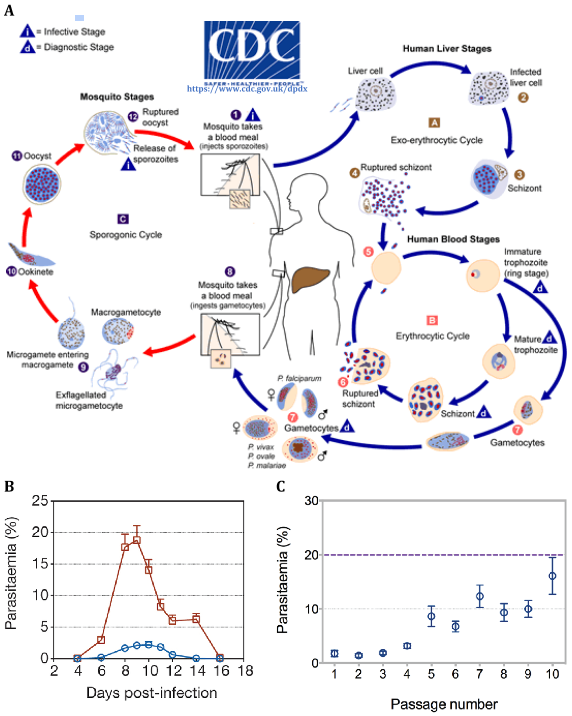
\includegraphics{images/background-spence2013.png}
\caption{Figure 1. Serial blood passage increases virulence of malaria
parasites.}
\end{figure}

    \hypertarget{is-the-transcriptome-of-a-mosquito-transmitted-parasite-different-from-one-which-has-not-passed-through-a-mosquito}{%
\subsection{Is the transcriptome of a mosquito-transmitted parasite
different from one which has not passed through a
mosquito?}\label{is-the-transcriptome-of-a-mosquito-transmitted-parasite-different-from-one-which-has-not-passed-through-a-mosquito}}

    The key reason for asking this question is that parasites which are
transmitted by mosquito (\textbf{MT}) are less virulent (severe/harmful)
than those which are serially blood passaged (\textbf{SBP}) in the
laboratory. \textit{Figure 1A} shows the malaria life cycle, the red part
highlighting the mosquito stage. \textit{Figure 1B} shows the difference
in virulence, measured by blood parasitemia (presence of parasites in
the blood), between mosquito-transmitted and serially blood passaged
parasites.

\textit{Figure 1C} shows that increasing numbers of blood passage post
mosquito transmission results in increasing virulence, back to around
20\% parasitemia. Subsequent mosquito transmission of high virulence
parasites render them low virulence again.

We hypothesise that parasites which have been through the mosquito are
somehow better able to control the mosquito immune system than those
which have not. This control of the immune system would result in lower
parasitemia because this is advantageous for the parasite. Too high a
parasitemia is bad for the mouse and therefore bad for the parasite.

\newpage

    \hypertarget{exercise-1}{%
\subsection{Exercise 1}\label{exercise-1}}

    In this tutorial, you will be analysing \textbf{five RNA samples}, each
of which has been sequenced on an Illumina HiSeq sequencing machine.
There are \textbf{two conditions}: serially blood-passaged parasites
(\textbf{SBP}) and mosquito transmitted parasites (\textbf{MT}). One
with \textbf{three biological replicates} (SBP), one with \textbf{two
biological replicates} (MT).

    \begin{longtable}[]{@{}ccc@{}}
\toprule
Sample name & Experimental condition & Replicate number\tabularnewline
\midrule
\endhead
MT1 & mosquito transmitted parasites & 1\tabularnewline
MT2 & mosquito transmitted parasites & 2\tabularnewline
SBP1 & serially blood-passaged parasites & 1\tabularnewline
SBP2 & serially blood-passaged parasites & 2\tabularnewline
SBP3 & serially blood-passaged parasites & 3\tabularnewline
\bottomrule
\end{longtable}

    \textbf{Check that you can see the tutorial FASTQ files in the
\texttt{data} directory.}

    \begin{tcolorbox}[breakable, size=fbox, boxrule=1pt, pad at break*=1mm,colback=cellbackground, colframe=cellborder]
\prompt{In}{incolor}{ }{\boxspacing}
\begin{Verbatim}[commandchars=\\\{\}]
ls data/*.fastq.gz
\end{Verbatim}
\end{tcolorbox}

    The FASTQ files contain the raw sequence reads for each sample. There
are four lines per read:

\begin{enumerate}
\def\labelenumi{\arabic{enumi}.}
\tightlist
\item
  Header
\item
  Sequence
\item
  Separator (usually a `+')
\item
  Encoded quality value
\end{enumerate}

    \textbf{Take a look at one of the FASTQ files.}

    \begin{tcolorbox}[breakable, size=fbox, boxrule=1pt, pad at break*=1mm,colback=cellbackground, colframe=cellborder]
\prompt{In}{incolor}{ }{\boxspacing}
\begin{Verbatim}[commandchars=\\\{\}]
zless data/MT1\PYZus{}1.fastq.gz \PY{p}{|} head
\end{Verbatim}
\end{tcolorbox}

    Find out more about FASTQ formats at
\url{https://en.wikipedia.org/wiki/FASTQ_format}.

    \hypertarget{questions}{%
\subsection{Questions}\label{questions}}

\hypertarget{q1-why-is-there-more-than-one-fastq-file-per-sample}{%
\subsubsection{Q1: Why is there more than one FASTQ file per
sample?}\label{q1-why-is-there-more-than-one-fastq-file-per-sample}}

\textit{Hint: think about why there is a MT1\_1.fastq.gz and a
MT1\_2.fastq.gz}

\hypertarget{q2-how-many-reads-were-generated-for-the-mt1-sample}{%
\subsubsection{Q2: How many reads were generated for the MT1
sample?}\label{q2-how-many-reads-were-generated-for-the-mt1-sample}}

\textit{Hint: we want the total number of reads from both files
(MT1\_1.fastq.gz and MT1\_2.fastq.gz) so perhaps think about the FASTQ
format and the number of lines for each read or whether there's anything
you can use in the FASTQ header to search and count\ldots{}}

Now let's move on to \textbf{\href{genome-mapping.ipynb}{mapping RNA-Seq reads to the genome
using HISAT2}}.


    % Add a bibliography block to the postdoc



\newpage





    \hypertarget{mapping-rna-seq-reads-to-the-genome-using-hisat2}{%
\section{Mapping RNA-Seq reads to the genome using
HISAT2}\label{mapping-rna-seq-reads-to-the-genome-using-hisat2}}

    \hypertarget{introduction}{%
\subsection{Introduction}\label{introduction}}

For this exercise, we have reduced the number of reads in each sample to
around 2.5 million to reduce the mapping time. However, this is
sufficient to detect most differentially expressed genes.

The objectives of this part of the tutorial are:

\begin{itemize}
\tightlist
\item
  \textit{use HISAT2 to build an index from the reference genome}
\item
  \textit{use HISAT2 to map RNA-Seq reads to the reference genome}
\end{itemize}

    \hypertarget{mapping-rna-seq-reads-to-a-genome}{%
\subsubsection{Mapping RNA-Seq reads to a
genome}\label{mapping-rna-seq-reads-to-a-genome}}

By this stage, you should have already performed a standard NGS quality
control check on your reads to see whether there were any issues with
the sample preparation or sequencing. In the interest of time, we won't
be doing that as part of this tutorial, but feel free to use the tools
from earlier modules to give that a go later if you have time.

Next, we map our RNA-Seq reads to a reference genome to get context.
This allows you to visually inspect your RNA-Seq data, identify
contamination, novel exons and splice sites as well as giving you an
overall feel for your transcriptome.

\hypertarget{hisat2}{%
\paragraph{HISAT2}\label{hisat2}}

To map the RNA-Seq reads from our five samples to the reference genome,
we will be using
\href{https://ccb.jhu.edu/software/hisat2/index.shtml}{HISAT2}, a fast
and sensitive splice-aware aligner. HISAT2 compresses the genome using
an indexing scheme based on the
\href{https://en.wikipedia.org/wiki/Burrows\%E2\%80\%93Wheeler_transform}{Burrows-Wheeler
transform (BWT)} and
\href{https://en.wikipedia.org/wiki/FM-index}{Ferragina-Manzini (FM)
index} to reduce the amount of space needed to store the genome. This
also makes the genome quick to search, using a whole-genome FM index to
anchor each alignment and then tens of thousands local FM indexes for
very rapid extensions of these alignments.

For more information, and to find the original version of \textit{Figure
2}, please see the HISAT paper:

\begin{quote}
\textbf{HISAT: a fast spliced aligner with low memory requirements}\\
Daehwan Kim, Ben Langmead and Steven L Salzberg\\
\textit{Nat Methods. 2015 Apr;12(4):357-60.
doi:\href{https://www.nature.com/articles/nmeth.3317}{10.1038/nmeth.3317}}
\end{quote}

HISAT2 is a splice-aware aligner which means it takes into account that
when a read is mapped it may be split across multiple exons with
(sometimes large) intronic gaps between aligned regions. As you can see
in \textit{Figure 2}, HISAT2 splits read alignments into five classes
based on the number of exons the read alignment is split across and the
length of the anchor (longest continuously mapped portion of a split
read):

\begin{itemize}
\tightlist
\item
  \textit{Aligns to a single exon (M)}
\item
  \textit{Alignment split across 2 exons with long anchors over 15bp
  (2M\_gt\_15)}
\item
  \textit{Alignment split across 2 exons with intermediate anchors between
  8bp and 15bp (2M\_8\_15)}
\item
  \textit{Alignment split across 2 exons with short anchors less than 7bp
  (2M\_1\_7)}
\item
  \textit{Alignment split across more than 2 exons (gt\_2M)}
\end{itemize}

HISAT2 used the global index to place the longest continuously mapped
portion of a read (\textit{anchor}). This information is then used to
identify the relevant local index. In most cases, HISAT2 will only need
to use a single local index to place the remaining portion of the read
without having to search the rest of the genome.

For the human genome, HISAT2 will build a single global index and 48,000
local FM indexes. Each of the local indexes represents a 64kb genomic
region. The majority of human introns are significantly shorter than
64kb, so \textgreater90\% of human introns fall into a single local
index. Moreover, each of the local indexes overlaps its neighbour by
\textasciitilde1kb which means that it also has the ability to detect
reads spanning multiple indexes.

    \begin{figure}[!h]
\centering
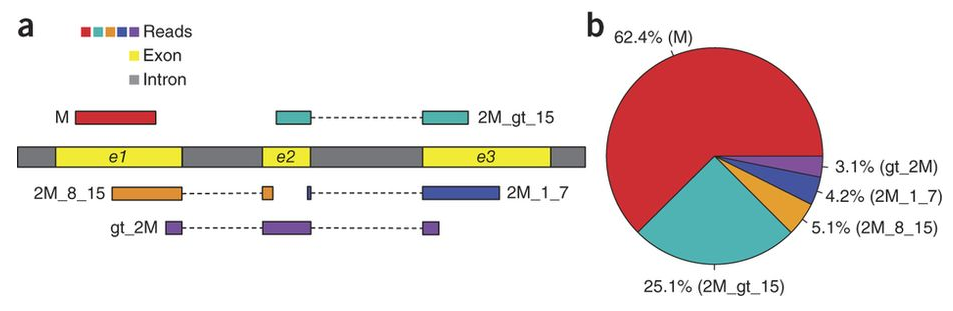
\includegraphics{images/split-reads.png}
\caption{Figure 2. Read types and their relative proportions from 20
million simulated 100-bp reads}
\end{figure}

    There are five HISAT2 RNA-seq read mapping categories: (i) M, exonic
read; (ii) 2M\_gt\_15, junction reads with long, \textgreater15-bp
anchors in both exons; (iii) 2M\_8\_15, junction reads with
intermediate, 8- to 15-bp anchors; (iv) 2M\_1\_7, junction reads with
short, 1- to 7-bp, anchors; and (v) gt\_2M, junction reads spanning more
than two exons (Figure 2A). Exoninc reads span only a single exon and
represent over 60\% of the read mappings in the 20 million 100-bp
simulated read dataset.

    \begin{center}\rule{0.5\linewidth}{0.5pt}\end{center}

    \hypertarget{exercise-2}{%
\subsection{Exercise 2}\label{exercise-2}}

    Be patient, each of the following steps will take a couple of minutes!

    \textbf{Look at the usage instructions for \texttt{hisat2-build}.}

    \begin{tcolorbox}[breakable, size=fbox, boxrule=1pt, pad at break*=1mm,colback=cellbackground, colframe=cellborder]
\prompt{In}{incolor}{ }{\boxspacing}
\begin{Verbatim}[commandchars=\\\{\}]
hisat2\PYZhy{}build \PYZhy{}h
\end{Verbatim}
\end{tcolorbox}

    This not only tells us the version of HISAT2 we're using (essential for
publication methods):

\begin{verbatim}
HISAT2 version 2.1.0 by Daehwan Kim (infphilo@gmail.com, http://www.ccb.jhu.edu/people/infphilo)
\end{verbatim}

But, that we also need to give \texttt{histat2-build} two pieces of
information:

\begin{verbatim}
Usage: hisat2-build [options]* <reference_in> <ht2_index_base>
\end{verbatim}

These are:

\begin{itemize}
\item
  \texttt{\textless{}reference\_in\textgreater{}}~\\
  location of our reference sequence file (PccAS\_v3\_genome.fa)
\item
  \texttt{\textless{}ht2\_index\_base\textgreater{}}~\\
  what we want to call our HISAT2 index files (PccAS\_v3\_hisat2.idx)
\end{itemize}

\newpage

    \textbf{Build a HISAT2 index for our \textit{Plasmodium chabaudi chabaudi
AS} (\textit{P. chabaudi}) reference genome using \texttt{hisat2-build}.}

    \begin{tcolorbox}[breakable, size=fbox, boxrule=1pt, pad at break*=1mm,colback=cellbackground, colframe=cellborder]
\prompt{In}{incolor}{ }{\boxspacing}
\begin{Verbatim}[commandchars=\\\{\}]
hisat2\PYZhy{}build data/PccAS\PYZus{}v3\PYZus{}genome.fa data/PccAS\PYZus{}v3\PYZus{}hisat2.idx
\end{Verbatim}
\end{tcolorbox}

    You can see the generated index files using:

    \begin{tcolorbox}[breakable, size=fbox, boxrule=1pt, pad at break*=1mm,colback=cellbackground, colframe=cellborder]
\prompt{In}{incolor}{ }{\boxspacing}
\begin{Verbatim}[commandchars=\\\{\}]
ls data/PccAS\PYZus{}v3\PYZus{}hisat2.idx*
\end{Verbatim}
\end{tcolorbox}

    \textbf{Look at the usage for \texttt{hisat2}.}

    \begin{tcolorbox}[breakable, size=fbox, boxrule=1pt, pad at break*=1mm,colback=cellbackground, colframe=cellborder]
\prompt{In}{incolor}{ }{\boxspacing}
\begin{Verbatim}[commandchars=\\\{\}]
hisat2 \PYZhy{}h
\end{Verbatim}
\end{tcolorbox}

    Here we can see that \texttt{hisat2} needs several bits of information
so that it can do the mapping:

\begin{verbatim}
hisat2 [options]* -x <ht2-idx> {-1 <m1> -2 <m2> | -U <r>} [-S <sam>]
\end{verbatim}

\begin{itemize}
\item
  \texttt{-x\ \textless{}ht2-idx\textgreater{}}~\\
  the prefix that we chose for our index files with
  \texttt{hisat2-build} (PccAS\_v3\_hisat2.idx)
\item
  \texttt{\{-1\ \textless{}m1\textgreater{}\ -2\ \textless{}m2\textgreater{}\ \textbar{}\ -U\ \textless{}r\textgreater{}\}}~\\
  the left (\texttt{-1}) and right (\texttt{-2}) read files for the
  sample (MT1\_1.fastq and MT1\_2.fastq respectively
\item
  \texttt{{[}-S\ \textless{}sam\textgreater{}{]}}~\\
  the name of the file we want to write the output alignment to
  (MT1.sam) as, by default, hisat2 will print the results to the
  terminal (stdout)
\end{itemize}

We will also be adding one more piece of information, the maximum intron
length (default 500,000 bases). For this analysis, we want to set the
maximum intron length to 10,000. We can do this by adding the option
\texttt{-\/-max-intronlen\ 10000}.

    \textbf{Map the reads for the MT1 sample using HISAT2.}

    \begin{tcolorbox}[breakable, size=fbox, boxrule=1pt, pad at break*=1mm,colback=cellbackground, colframe=cellborder]
\prompt{In}{incolor}{ }{\boxspacing}
\begin{Verbatim}[commandchars=\\\{\}]
hisat2 \PYZhy{}\PYZhy{}max\PYZhy{}intronlen \PY{l+m}{10000} \PYZhy{}x data/PccAS\PYZus{}v3\PYZus{}hisat2.idx \PY{l+s+se}{\PYZbs{}}
\PYZhy{}1 data/MT1\PYZus{}1.fastq.gz \PYZhy{}2 data/MT1\PYZus{}2.fastq.gz \PYZhy{}S data/MT1.sam
\end{Verbatim}
\end{tcolorbox}

    HISAT2 has written the alignment in SAM format. This is a format which
allows humans to look at our alignments. However, we need to convert the
SAM file to its binary version, a BAM file. We do this for several
reasons. Mainly we do it because most downstream programs require our
alignments to be in BAM format and not SAM format. However, we also do
it because the BAM file is smaller and so takes up less (very precious!)
storage space. For more information, see the format guide:
\url{http://samtools.github.io/hts-specs/SAMv1.pdf}.

    \textbf{Convert the SAM file to a BAM file.}

    \begin{tcolorbox}[breakable, size=fbox, boxrule=1pt, pad at break*=1mm,colback=cellbackground, colframe=cellborder]
\prompt{In}{incolor}{ }{\boxspacing}
\begin{Verbatim}[commandchars=\\\{\}]
samtools view \PYZhy{}b \PYZhy{}o data/MT1.bam data/MT1.sam
\end{Verbatim}
\end{tcolorbox}

\newpage

    We now need to sort the BAM file ready for indexing. When we aligned our
reads with HISAT2, alignments were produced in the same order as the
sequences in our FASTQ files. To index the BAM file, we need the
alignments ordered by their respective positions in the reference
genome. We can do this using \texttt{samtools\ sort} to sort the
alignments by their co-ordinates for each chromosome.

    \textbf{Sort the BAM file.}

    \begin{tcolorbox}[breakable, size=fbox, boxrule=1pt, pad at break*=1mm,colback=cellbackground, colframe=cellborder]
\prompt{In}{incolor}{ }{\boxspacing}
\begin{Verbatim}[commandchars=\\\{\}]
samtools sort \PYZhy{}o data/MT1\PYZus{}sorted.bam data/MT1.bam
\end{Verbatim}
\end{tcolorbox}

    Next, we need to index our BAM file. This makes searching the alignments
much more efficient. It allows programs like IGV (which we will be using
to visualise the alignment) to quickly get the alignments that overlap
the genomic regions you're looking at. We can do this with
\texttt{samtools\ index} which will generate an index file with the
extension \textbf{.bai}.

    \textbf{Index the BAM file so that it can be read efficiently by IGV.}

    \begin{tcolorbox}[breakable, size=fbox, boxrule=1pt, pad at break*=1mm,colback=cellbackground, colframe=cellborder]
\prompt{In}{incolor}{ }{\boxspacing}
\begin{Verbatim}[commandchars=\\\{\}]
samtools index data/MT1\PYZus{}sorted.bam
\end{Verbatim}
\end{tcolorbox}

    \textbf{Now, repeat this process of mapping, converting (SAM to BAM),
sorting and indexing with the reads from the MT2 sample. You can run the
previous steps as a single command.}

    hisat2 --max-intronlen 10000 -x data/PccAS\_v3\_hisat2.idx\\
-1 data/MT2\_1.fastq.gz -2 data/MT2\_2.fastq.gz\\
\textbar{} samtools view -b -\\
\textbar{} samtools sort -o data/MT2\_sorted.bam -\\
\&\& samtools index data/MT2\_sorted.bam

    \textbf{Let's not forget our SBP samples. We've already provided the BAM
files for these samples. Please check that you can see the BAM files
before continuing.}

    \begin{tcolorbox}[breakable, size=fbox, boxrule=1pt, pad at break*=1mm,colback=cellbackground, colframe=cellborder]
\prompt{In}{incolor}{ }{\boxspacing}
\begin{Verbatim}[commandchars=\\\{\}]
ls \PYZhy{}al data/SBP*.bam
\end{Verbatim}
\end{tcolorbox}

    You should see three files:

\begin{verbatim}
  data/SBP1_sorted.bam
  data/SBP2_sorted.bam
  data/SBP3_sorted.bam
\end{verbatim}

\textbf{If you can't see these files, please let your instructor know!!}

We've previously shown you how to run HISAT2 and samtools with
individual and one-line commands. For the SBP samples, a bash script was
used to generate our genome alignments prior to this tutorial.

To take a look at the script you can run:

\begin{verbatim}
less data/map_SBP_samples.sh
\end{verbatim}

If you have time at the end of the tutorial, feel free to take a closer
look at the script and a more detailed breakdown of what it does in
\href{running-commands-on-multiple-samples.ipynb}{Running commands on
multiple samples}. Bash scripts and loops are a useful way of automating
an analysis and running the same commands for multiple samples. Imagine
if you had 50 samples and not 5! In truth, you'd probably want to run
that many samples on a compute cluster, in parallel. But that's outside
the scope of this tutorial.

\newpage

    \hypertarget{questions}{%
\subsection{Questions}\label{questions}}

    \hypertarget{q1-how-many-index-files-were-generated-when-you-ran-hisat2-build}{%
\subsubsection{\texorpdfstring{Q1: How many index files were generated
when you ran
\texttt{hisat2-build?}}{Q1: How many index files were generated when you ran hisat2-build?}}\label{q1-how-many-index-files-were-generated-when-you-ran-hisat2-build}}

\textit{Hint: look for the files with the \texttt{.ht2} extension}

\hypertarget{q2-what-was-the-overall-alignment-rate-for-each-of-the-mt-samples-mt1-and-mt2-to-the-reference-genome}{%
\subsubsection{\texorpdfstring{Q2: What was the \textit{overall alignment
rate} for each of the MT samples (MT1 and MT2) to the reference
genome?}{Q2: What was the overall alignment rate for each of the MT samples (MT1 and MT2) to the reference genome?}}\label{q2-what-was-the-overall-alignment-rate-for-each-of-the-mt-samples-mt1-and-mt2-to-the-reference-genome}}

\textit{Hint: look at the the output from the \texttt{hisat2} commands}

\hypertarget{q3-how-many-mt1-and-mt2-reads-were-not-aligned-to-the-reference-genome}{%
\subsubsection{Q3: How many MT1 and MT2 reads were not aligned to the
reference
genome?}\label{q3-how-many-mt1-and-mt2-reads-were-not-aligned-to-the-reference-genome}}

\textit{Hint: look at the the output from the \texttt{hisat2} commands,
you're looking for reads (not read pairs) which have aligned 0 times
(remember that one read from a pair may map even if the other doesn't)}

    % Add a bibliography block to the postdoc

\newpage

    \hypertarget{visualising-transcriptomes-with-igv}{%
\section{Visualising transcriptomes with
IGV}\label{visualising-transcriptomes-with-igv}}

    \hypertarget{introduction}{%
\subsection{Introduction}\label{introduction}}

\href{https://software.broadinstitute.org/software/igv/}{Integrative
Genome Viewer} (\textbf{IGV}) allows us to visualise genomic datasets.
We have provided a quick start guide which contains the information you
need to complete \hyperref[exercise-3]{Exercise 3}. There is also an IGV
user guide online which contains more information on all of the IGV
features and functions:
http://software.broadinstitute.org/software/igv/UserGuide.

The objectives of this part of the tutorial are:

\begin{itemize}
\tightlist
\item
  \textit{load a reference genome into IGV and navigate the genome}
\item
  \textit{load an annotation file into IGV and explore gene structure}
\item
  \textit{load read alignments into IGV and inspect read alignments}
\end{itemize}

    \begin{center}\rule{0.5\linewidth}{0.5pt}\end{center}

    \hypertarget{exercise-3}{%
\subsection{Exercise 3}\label{exercise-3}}

First, we will use \texttt{samtools} to create an index for the \textit{P.
chabaudi} reference genome, which IGV will use to traverse the genome.
This index file will have the extension \textbf{.fai} and should always
be in the same directory as the reference genome.

    \textbf{First, index the genome fasta file (required by IGV).}

    \begin{tcolorbox}[breakable, size=fbox, boxrule=1pt, pad at break*=1mm,colback=cellbackground, colframe=cellborder]
\prompt{In}{incolor}{ }{\boxspacing}
\begin{Verbatim}[commandchars=\\\{\}]
samtools faidx data/PccAS\PYZus{}v3\PYZus{}genome.fa
\end{Verbatim}
\end{tcolorbox}

    \textbf{Now, start IGV.}

    \begin{tcolorbox}[breakable, size=fbox, boxrule=1pt, pad at break*=1mm,colback=cellbackground, colframe=cellborder]
\prompt{In}{incolor}{ }{\boxspacing}
\begin{Verbatim}[commandchars=\\\{\}]
igv \PY{p}{\PYZam{}}
\end{Verbatim}
\end{tcolorbox}

    This will open the IGV main window. Now, we need to tell IGV which
genome we want to use. IGV has many pre-loaded genomes available, but
\textit{P. chabaudi} is not one of them. This means we will need to load
our genome from a file.

\textbf{Load your reference genome into IGV. Go to ``\textit{Genomes
-\textgreater{} Load Genome from File\ldots{}}''. Select
``PccAS\_v3\_genome.fa'' and click ``\textit{Open}''. For more
information, see
\href{https://github.com/sanger-pathogens/pathogen-informatics-training/blob/master/Notebooks/IGV/index.ipynb}{Loading
a reference genome} in our quick start guide.}

\newpage

We not only want to see where our reads have mapped, but what genes they
have mapped to. For this, we have an annotation file in
\href{https://www.ensembl.org/info/website/upload/gff3.html}{GFF3
format}. This contains a list of features, their co-ordinates and
orientations which correspond to our reference genome.

    \begin{figure}[!h]
\centering
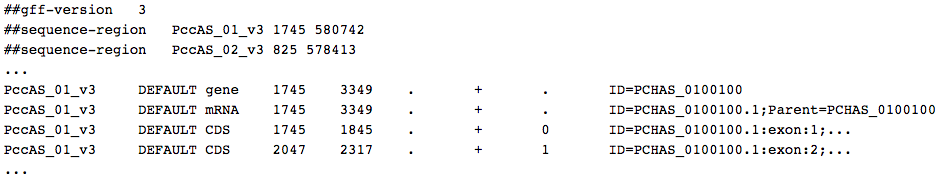
\includegraphics{images/PccAS_v3_gff3.png}
\caption{Example from PccAS\_v3 GFF3}
\end{figure}

    \textbf{Load your annotation file into IGV. Go to "``File
-\textgreater{} Load from File\ldots{}''. Select ``PccAS\_v3.gff3'' and
click ``\textit{Open}''. For more information, see
\href{https://github.com/sanger-pathogens/pathogen-informatics-training/blob/master/Notebooks/IGV/index.ipynb}{Loading
gene annotations} in our quick start guide.}

This will load a new track called ``PccAS\_v3.gff3''. The track is
currently shown as a density plot. You will need to zoom in to see
individual genes.

\textbf{Search for the gene PCHAS\_0505200 by typing ``PCHAS\_0505200''
in the search box to zoom in and centre the view on PCHAS\_0505200.}

    \begin{figure}[!h]
\centering
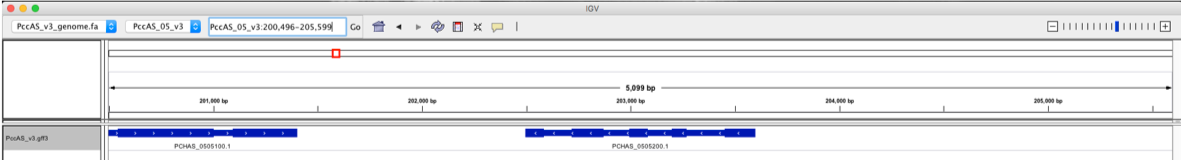
\includegraphics{images/igv-gene.png}
\caption{IGV - PCHAS\_0505200}
\end{figure}

    \textbf{To get a clearer view of the gene structure, right click on the
annotation track and click ``Expanded''.}

    \begin{figure}[!h]
\centering
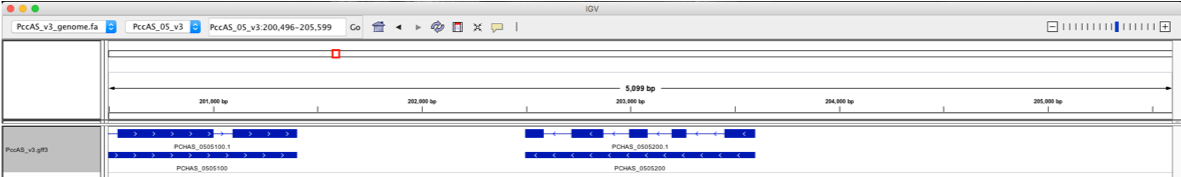
\includegraphics{images/igv-gene-structure.png}
\caption{IGV - PCHAS\_0505200 expanded}
\end{figure}

    In the annotation track, genes are presented as blue boxes and lines.
These boxes represent exons, while the lines represent intronic regions.
Arrows indicate the direction (or strand) of transcription for each of
the genes. Now we have our genome and its annotated features, we just
need the read alignments for our five samples.

\newpage

\textbf{Load your alignment file for the MT1 sample into IGV. Go to
"``File -\textgreater{} Load from File\ldots{}''. Select
``\textit{MT1\_sorted.bam}'' and click ``\textit{Open}''. For more
information, see
\href{https://github.com/sanger-pathogens/pathogen-informatics-training/blob/master/Notebooks/IGV/index.ipynb}{Loading
alignment files} in our quick start guide.}

\textit{Note: BAM files and their corresponding index files must be in the
same directory for IGV to load them properly.}

    \begin{figure}[!h]
\centering
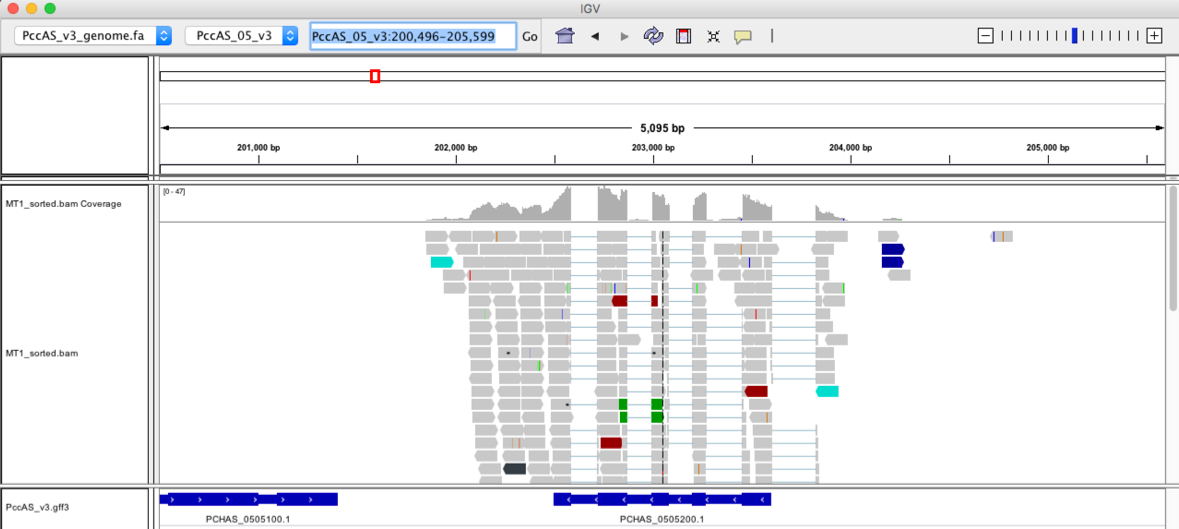
\includegraphics{images/igv-mt1.png}
\caption{IGV - MT1 read alignment}
\end{figure}

    This will load a new track called ``MT1\_sorted.bam'' which contains the
read alignments for the MT1 sample. We can change how we visualise our
data by altering the view options. By default, IGV will display reads
individually so they are compactly arranged. If you were to hover over a
read in the default view, you will only get the details for that read.
However, if we change our view so that the reads are visualised as
pairs, the read pairs will be joined together by line and when we hover
over either of the reads, we will get information about both of the
reads in that pair.

    \textbf{To view our reads as pairs, right click on the MT1\_sorted.bam
alignment track and click ``View as pairs''.}

    \begin{figure}[!h]
\centering
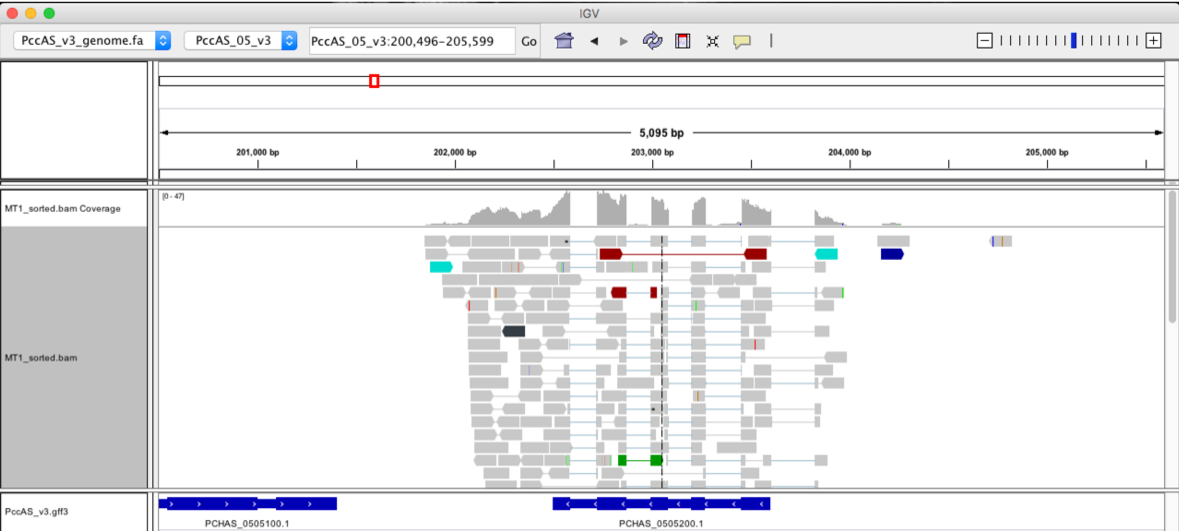
\includegraphics{images/igv-mt1-paired.png}
\caption{IGV - paired view}
\end{figure}

\newpage

    \textbf{To condense the alignment, right click on the MT1\_sorted.bam
alignment track and click ``Squished''.}

    \begin{figure}[!h]
\centering
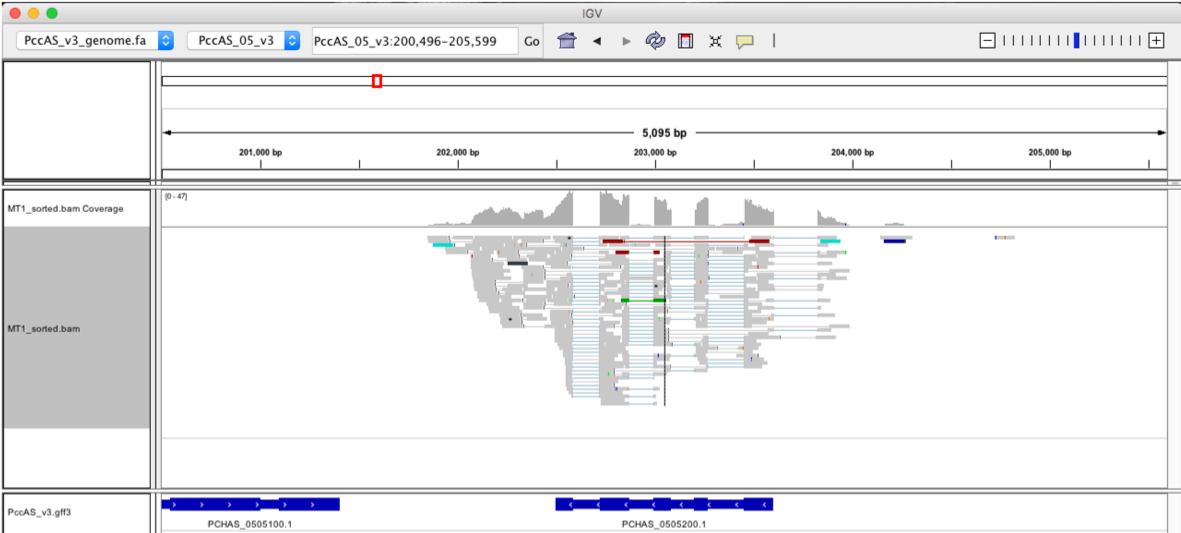
\includegraphics{images/igv-mt1-squished.png}
\caption{IGV - squished view}
\end{figure}

    For more information on sorting, grouping and visualising read
alignments, see the
\href{http://software.broadinstitute.org/software/igv/UserGuide}{IGV
user guide}.

\textbf{Load the remaining sorted BAM files for the MT2 sample and the
three SBP samples.}

\textbf{Using the search box in the toolbar, go to PCHAS\_1409500. For
more information, see
\href{https://github.com/sanger-pathogens/pathogen-informatics-training/blob/master/Notebooks/IGV/index.ipynb}{Jump
to gene or locus} in our quick start guide.}

    \begin{figure}[!h]
\centering
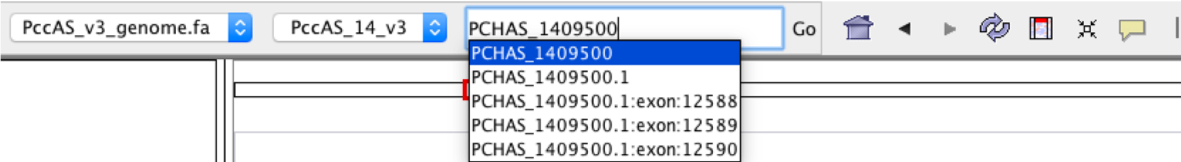
\includegraphics{images/igv-search-pchas1409500.png}
\caption{IGV - search PCHAS\_1409500}
\end{figure}

    The first thing to look at is the coverage range for this viewing window
on the left-hand side. The three SBP samples have 2-3 times more reads
mapping to this gene than the two MT samples. While at first glance it
may seem like this gene may be differentially expressed between the two
conditions, remember that some samples may have been sequenced to a
greater depth than others. So, if a sample has been sequenced to a
greater depth we would expect more reads to map in general.

    \begin{figure}[!h]
\centering
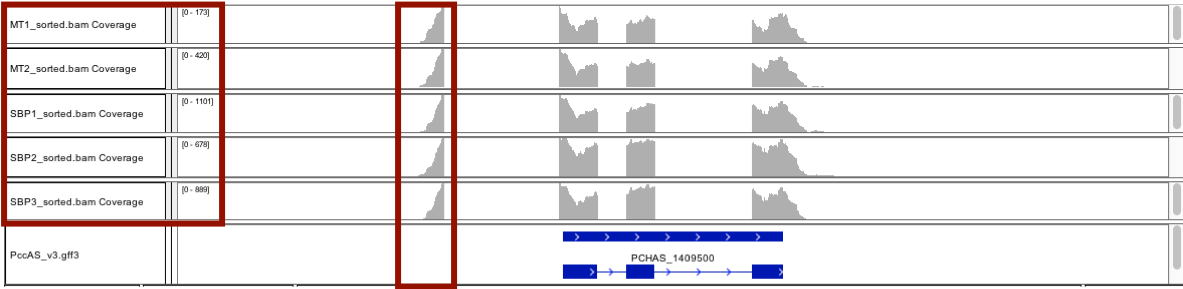
\includegraphics{images/igv-coverage-pchas1409500.png}
\caption{IGV - coverage PCHAS\_1409500}
\end{figure}

\newpage

    From the gene annotation at the bottom we can also see that there are
three annotated exon/CDS features for this gene. However, the coverage
plot suggests there may be a fourth unannotated exon which, given the
direction of the gene, could suggest a 5' untranslated region (UTR).
Note the clean drop off of the coveraged at around position 377,070.

    \begin{center}\rule{0.5\linewidth}{0.5pt}\end{center}

    \hypertarget{questions}{%
\subsection{Questions}\label{questions}}

\hypertarget{q1-how-many-cds-features-are-there-in-pchas_1402500}{%
\subsubsection{Q1: How many CDS features are there in
``PCHAS\_1402500''?}\label{q1-how-many-cds-features-are-there-in-pchas_1402500}}

\textit{Hint: Look at
\href{https://github.com/sanger-pathogens/pathogen-informatics-training/blob/master/Notebooks/IGV/index.ipynb}{Jump
to gene or locus} in our quick start guide.}

\hypertarget{q2-does-the-rna-seq-mapping-agree-with-the-gene-model-in-blue}{%
\subsubsection{Q2: Does the RNA-seq mapping agree with the gene model in
blue?}\label{q2-does-the-rna-seq-mapping-agree-with-the-gene-model-in-blue}}

\textit{Hint: Look at the coverage track and split read alignments.}

\hypertarget{q3-do-you-think-this-gene-is-differentially-expressed-and-is-looking-at-the-coverage-plots-alone-a-reliable-way-to-assess-differential-expression}{%
\subsubsection{Q3: Do you think this gene is differentially expressed
and is looking at the coverage plots alone a reliable way to assess
differential
expression?}\label{q3-do-you-think-this-gene-is-differentially-expressed-and-is-looking-at-the-coverage-plots-alone-a-reliable-way-to-assess-differential-expression}}

\textit{Hint: Look at the coverage similarities/differences between the MT
and SBP samples.}

    % Add a bibliography block to the postdoc



\newpage





    \hypertarget{transcript-quantification-with-kallisto}{%
\section{Transcript quantification with
Kallisto}\label{transcript-quantification-with-kallisto}}

    \hypertarget{introduction}{%
\subsection{Introduction}\label{introduction}}

After visually inspecting the genome alignment, the next step in a
typical RNA-Seq analysis is to estimate transcript abundance. To do
this, reads are assigned to the transcripts they came from. These
assignments are then used to quantify gene or transcript abundance
(expression level).

For this tutorial, we are using
\href{https://pachterlab.github.io/kallisto/}{Kallisto} to assign reads
to a set of transcript sequences and quantify transcript abundance.
Kallisto does not assemble transcripts and cannot identify novel
isoforms. So, when a reference transcriptome isn't available, the
transcripts will need to be assembled \textit{de novo} from the reads.
However, for this tutorial, we already have a reference transcriptome
available.

The objectives of this part of the tutorial are:

\begin{itemize}
\tightlist
\item
  use Kallisto to index a transcriptome
\item
  use Kallisto to estimate transcript abundance
\end{itemize}

    \hypertarget{quantifying-transcripts-with-kallisto}{%
\subsubsection{Quantifying transcripts with
Kallisto}\label{quantifying-transcripts-with-kallisto}}

Many of the existing methods used for estimating transcript abundance
are \textbf{alignment-based}. This means they rely on mapping reads onto
the reference genome. The gene expression levels are then calculated by
counting the number of reads overlapping the transcripts. However, read
alignment is a computationally and time intensive process. So, in this
tutorial, we will be running
\href{https://pachterlab.github.io/kallisto/}{Kallisto} which uses a
fast, \textbf{alignment-free} method for transcript quantification.

\begin{quote}
\textbf{Near-optimal probabilistic RNA-seq quantification}\\
Nicolas L Bray, Harold Pimentel, Páll Melsted and Lior Pachter\\
\textit{Nat Biotechnol. 2016 May;34(5):525-7. doi:
\href{https://www.nature.com/articles/nbt.3519}{10.1038/nbt.3519}}
\end{quote}

Kallisto uses \textbf{pseudoalignment} to make it
efficient. Rather than looking at where the reads map, Kallisto uses the
\textit{compatibility} between the reads and transcripts to estimate
transcript abundance. Thus, most transcript quantification with Kallisto
can be done on a simple laptop (Figure 3).

    \begin{figure}[!h]
\centering
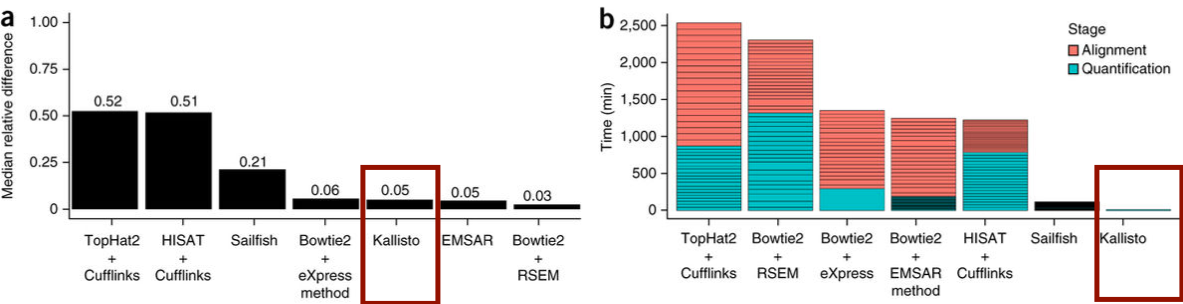
\includegraphics{images/kallisto-performance.png}
\caption{Figure 3. Performance of kallisto and other methods}
\end{figure}

    \textbf{Figure 3. Performance of kallisto and other methods}\\
\textit{(a) Accuracy of kallisto, Cufflinks, Sailfish, EMSAR, eXpress and
RSEM on 20 RSEM simulations of 30 million 75-bp paired-end reads. (b)
Total running time in minutes for processing the 20 simulated data sets
of 30 million paired-end reads described in a. Please see the
\href{https://www.nature.com/articles/nbt.3519}{Kallisto publication}
for original figure and more information.}

\newpage

    \hypertarget{step-1-building-a-kallisto-index}{%
\paragraph{Step 1: building a Kallisto
index}\label{step-1-building-a-kallisto-index}}

As with alignment-based methods, Kallisto needs an index. To generate
the index, Kallisto first builds a transcriptome de Bruijn Graph (T-BDG)
from all of the \textit{k}-mers (short sequences of \textit{k} nucleotides)
that it finds in the transcriptome. Each node in the graph corresponds
to a \textit{k}-mer and each transcript is represented by its path through
the graph. Using these paths, each \textit{k}-mer is assigned a
\textit{k}-compatibility class. Some \textit{k}-mers will be redundant
i.e.~shared by the same transcripts. These are skipped to make the index
compact and quicker to search. A great worked example of this process
can be found
\href{http://bioinfo.iric.ca/understanding-how-kallisto-works/}{here}.

The command \texttt{kallisto\ index} can be used to build a Kallisto
index from transcript sequences.

    \begin{tcolorbox}[breakable, size=fbox, boxrule=1pt, pad at break*=1mm,colback=cellbackground, colframe=cellborder]
\prompt{In}{incolor}{ }{\boxspacing}
\begin{Verbatim}[commandchars=\\\{\}]
kallisto index
\end{Verbatim}
\end{tcolorbox}

    Here we can see the version of Kallisto that we're using (useful for
publication methods) and the information that we'll need to give
\texttt{kallisto\ index}. The only information we need to give
\texttt{kallisto\ index} is the location of our transcript sequences
(PccAS\_v3\_transcripts.fa). However, it's useful to have a meaningful
filename for the resulting index. We can add this by using the option
\texttt{-i} which expects a value, our index prefix
(PccAS\_v3\_kallisto).

    \hypertarget{step-2-estimating-transcript-abundance}{%
\paragraph{Step 2: estimating transcript
abundance}\label{step-2-estimating-transcript-abundance}}

With this Kallisto index, you can use \texttt{kallisto\ quant} to
estimate transcript abundances. You will need to run this command
separately for each sample.

    \begin{tcolorbox}[breakable, size=fbox, boxrule=1pt, pad at break*=1mm,colback=cellbackground, colframe=cellborder]
\prompt{In}{incolor}{ }{\boxspacing}
\begin{Verbatim}[commandchars=\\\{\}]
kallisto quant
\end{Verbatim}
\end{tcolorbox}

    We can see that \texttt{kallisto\ quant} needs us to tell it where our
sample read are. Although we don't have to, it's usually a good idea to
keep the results of each quantification in a different directory. This
is because the output filename are always the same
(e.g.~abundances.tsv). If we ran a second analysis, these could get
overwritten. To use a different output directory, we can use the
\texttt{-o} option. We will also be using the \texttt{-b} option for
bootstrapping.

    \hypertarget{bootstrapping}{%
\paragraph{Bootstrapping}\label{bootstrapping}}

Not all reads will be assigned unambiguously to a single transcript.
This means there will be ``noise'' in our abundance estimates where
reads can be assigned to multiple transcripts. Kallisto quantifies the
uncertainty in its abundance estimates using random resampling and
replacement. This process is called \textbf{bootstrapping} and indicates
how reliable the expression estimates are from the observed
pseudoalignment. Bootstrap values can be used downstream to distinguish
the technical variability from the biological variability in your
experiment.

    \begin{center}\rule{0.5\linewidth}{0.5pt}\end{center}

    \hypertarget{exercise-4}{%
\subsection{Exercise 4}\label{exercise-4}}

    \textbf{Build an index called \textit{PccAS\_v3\_kallisto} from transcript
sequences in \textit{PccAS\_v3\_transcripts.fa}.}

    \begin{tcolorbox}[breakable, size=fbox, boxrule=1pt, pad at break*=1mm,colback=cellbackground, colframe=cellborder]
\prompt{In}{incolor}{ }{\boxspacing}
\begin{Verbatim}[commandchars=\\\{\}]
kallisto index \PYZhy{}i data/PccAS\PYZus{}v3\PYZus{}kallisto data/PccAS\PYZus{}v3\PYZus{}transcripts.fa
\end{Verbatim}
\end{tcolorbox}

\newpage

    \textbf{Quantify the transcript expression levels for the MT1 sample
with 100 bootstrap samples and calling the output directory \textit{MT1}.}

    \begin{tcolorbox}[breakable, size=fbox, boxrule=1pt, pad at break*=1mm,colback=cellbackground, colframe=cellborder]
\prompt{In}{incolor}{ }{\boxspacing}
\begin{Verbatim}[commandchars=\\\{\}]
kallisto quant \PYZhy{}i data/PccAS\PYZus{}v3\PYZus{}kallisto \PYZhy{}o data/MT1 \PYZhy{}b \PY{l+m}{100} \PY{l+s+se}{\PYZbs{}}
data/MT1\PYZus{}1.fastq.gz data/MT1\PYZus{}2.fastq.gz
\end{Verbatim}
\end{tcolorbox}

    You'll find your Kallisto results in a new output directory which we
called \textbf{MT1}. Let's take a look.

    \begin{tcolorbox}[breakable, size=fbox, boxrule=1pt, pad at break*=1mm,colback=cellbackground, colframe=cellborder]
\prompt{In}{incolor}{ }{\boxspacing}
\begin{Verbatim}[commandchars=\\\{\}]
ls data/MT1
\end{Verbatim}
\end{tcolorbox}

    Running \texttt{kallisto\ quant} generated three output files in our
\texttt{MT1} folder:

\begin{itemize}
\item
  \textbf{abundance.h5}\\
  HDF5 binary file containing run info, abundance esimates, bootstrap
  estimates, and transcript length information length.
\item
  \textbf{abundance.tsv}\\
  Plain text file containing abundance estimates (doesn't contain
  bootstrap estimates).
\item
  \textbf{run\_info.json}\\
  JSON file containing information about the run.
\end{itemize}

\textit{Note: when the number of bootstrap values (\texttt{-b}) is very
high, Kallisto will generate a large amount of data. To help, it outputs
bootstrap results in HDF5 format (abundance.h5). This file can be read
directly by \href{https://pachterlab.github.io/sleuth}{sleuth}.}

In the \textbf{MT1/abundance.tsv} file we have the abundance estimates
for each gene for the MT1 sample. Let's take a quick look.

    \begin{tcolorbox}[breakable, size=fbox, boxrule=1pt, pad at break*=1mm,colback=cellbackground, colframe=cellborder]
\prompt{In}{incolor}{ }{\boxspacing}
\begin{Verbatim}[commandchars=\\\{\}]
head data/MT1/abundance.tsv
\end{Verbatim}
\end{tcolorbox}

    In \textbf{MT1/abundance.tsv} there are five columns which give us
information about the transcript abundances for our MT1 sample.

\begin{itemize}
\item
  \textbf{target\_id}\\
  Unique transcript identifier.
\item
  \textbf{length}\\
  Number of bases found in exons.
\item
  \textbf{eff\_length}\\
  \textit{Effective length}. Uses fragment length distribution to
  determine the effective number of positions that can be sampled on
  each transcript.
\item
  \textbf{est\_counts}\\
  Estimated counts*. This may not always be an integer as reads which
  map to multiple transcripts are fractionally assigned to each of the
  corresponding transcripts.
\item
  \textbf{tpm}\\
  \textit{Transcripts per million}. Normalised value accounting for length
  and sequence depth bias.
\end{itemize}

In the last column we have our normalised abundance value for each gene.
These are our transcripts per million or TPM. If you have time at the
end of this tutorial, see our \href{normalisation.ipynb}{normalisation
guide} which covers common normalisation methods and has a bonus
exercise.

\newpage

To get the result for a specific gene, we can use \texttt{grep}.

    \begin{tcolorbox}[breakable, size=fbox, boxrule=1pt, pad at break*=1mm,colback=cellbackground, colframe=cellborder]
\prompt{In}{incolor}{ }{\boxspacing}
\begin{Verbatim}[commandchars=\\\{\}]
grep PCHAS\PYZus{}0100100 data/MT1/abundance.tsv
\end{Verbatim}
\end{tcolorbox}

    If we wanted to get the TPM value for a particular gene, we can use
\texttt{awk}.

    \begin{tcolorbox}[breakable, size=fbox, boxrule=1pt, pad at break*=1mm,colback=cellbackground, colframe=cellborder]
\prompt{In}{incolor}{ }{\boxspacing}
\begin{Verbatim}[commandchars=\\\{\}]
awk \PYZhy{}F\PY{l+s+s2}{\PYZdq{}\PYZbs{}t\PYZdq{}} \PY{l+s+s1}{\PYZsq{}\PYZdl{}1==\PYZdq{}PCHAS\PYZus{}0100100\PYZdq{} \PYZob{}print \PYZdl{}5\PYZcb{}\PYZsq{}} data/MT1/abundance.tsv
\end{Verbatim}
\end{tcolorbox}

    \textbf{Use \texttt{kallisto\ quant} four more times, for the MT2 sample
and the three SBP samples.}

    \begin{center}\rule{0.5\linewidth}{0.5pt}\end{center}

    \hypertarget{questions}{%
\subsection{Questions}\label{questions}}

\hypertarget{q1-what-k-mer-length-was-used-to-build-the-kallisto-index}{%
\subsubsection{\texorpdfstring{Q1: What \textit{k}-mer length was used to
build the Kallisto
index?}{Q1: What k-mer length was used to build the Kallisto index?}}\label{q1-what-k-mer-length-was-used-to-build-the-kallisto-index}}

\textit{Hint: look at the terminal output from \texttt{kallisto\ index}}

\hypertarget{q2-how-many-transcript-sequences-are-there-in-pccas_v3_transcripts.fa}{%
\subsubsection{\texorpdfstring{Q2: How many transcript sequences are
there in
\textit{PccAS\_v3\_transcripts.fa}?}{Q2: How many transcript sequences are there in PccAS\_v3\_transcripts.fa?}}\label{q2-how-many-transcript-sequences-are-there-in-pccas_v3_transcripts.fa}}

\textit{Hint: you can use \texttt{grep} or look at the terminal output
from \texttt{kallisto\ quant} or in the run\_info.json files}

\hypertarget{q3-what-is-the-transcripts-per-million-tpm-value-for-pchas_1402500-in-each-of-the-samples}{%
\subsubsection{Q3: What is the transcripts per million (TPM) value for
PCHAS\_1402500 in each of the
samples?}\label{q3-what-is-the-transcripts-per-million-tpm-value-for-pchas_1402500-in-each-of-the-samples}}

\textit{Hint: use \texttt{grep} to look at the abundance.tsv files}

\hypertarget{q4-do-you-think-pchas_1402500-is-differentially-expressed}{%
\subsubsection{Q4: Do you think PCHAS\_1402500 is differentially
expressed?}\label{q4-do-you-think-pchas_1402500-is-differentially-expressed}}

    % Add a bibliography block to the postdoc



\newpage

    \hypertarget{identifying-differentially-expressed-genes-with-sleuth}{%
\section{Identifying differentially expressed genes with
Sleuth}\label{identifying-differentially-expressed-genes-with-sleuth}}

    \hypertarget{introduction}{%
\subsection{Introduction}\label{introduction}}

In the previous sections, we have quantified our transcript abundance
and looked at why counts are normalised. In this section, you will be
using \href{https://pachterlab.github.io/sleuth}{sleuth} to do some
simple quality checks and get a first look at the results.

The objectives of this part of the tutorial are:

\begin{itemize}
\tightlist
\item
  use sleuth to perform quality control checks
\item
  use sleuth to identify differentially expressed (DE) transcripts
\item
  use sleuth to investigate DE transcripts
\end{itemize}

\hypertarget{differential-expression-analysis-dea}{%
\subsubsection{Differential expression analysis
(DEA)}\label{differential-expression-analysis-dea}}

Differential expression analysis tries to identify genes whose
expression levels differ between experimental conditions. We don't
normally have enough replicates to do traditional tests of significance
for RNA-Seq data. So, most methods look for outliers in the relationship
between average abundance and fold change and assume most genes are not
differentially expressed.

Rather than just using a fold change threshold to determine which genes
are differentially expressed, DEAs use a variety of statistical tests
for significance. These tests give us a \textbf{p-value} which is an
estimate of how often your observations would occur by chance.

However, we perform these comparisons for each one of the thousands of
genes/transcripts in our dataset. A p-value of 0.01 estimates a
probability of 1\% for seeing our observation just by chance. In an
experiment like ours with 5,000 genes we would expect 5 genes to be
significantly differentially expressed by chance (i.e.~even if there
were no difference between our conditions). Instead of using a p-value
we use a \textbf{q-value} to account for multiple testing
and adjusts the p-value accordingly.

\hypertarget{sleuth}{%
\subsubsection{sleuth}\label{sleuth}}

\href{https://pachterlab.github.io/sleuth}{sleuth} is a companion tool
for \href{https://pachterlab.github.io/kallisto}{Kallisto}. Unlike most
other tools, sleuth can utilize the technical variation information
generated by Kallisto so that you can look at both the technical and
biological variation in your dataset.

For the DEA, sleuth essentially tests two models, one which assumes that
the abundances are equal between the two conditions (reduced) and one
that does not (full). To identify DE transcripts it identifies those
with a significantly better fit to the ``full'' model. For more
information on sleuth and how it works, see Lior Pachter's blog post
\textbf{A sleuth for RNA-Seq}
(https://liorpachter.wordpress.com/2015/08/17/a-sleuth-for-rna-seq/).

sleuth is written in the \href{https://www.r-project.org/}{R}
statistical programming language, as is almost all RNA-Seq analysis
software. Helpfully, it produces a web page that allows interactive
graphical analysis of the data. However, we strongly recommend learning
R for anyone doing a significant amount of RNA-seq analysis. It is
nowhere near as hard to get started with as full-blown programming
languages such as Perl or Python!

\newpage

    \hypertarget{exercise-5}{%
\subsection{Exercise 5}\label{exercise-5}}

    For this tutorial, we've provided a series of R commands as an R script
that will get sleuth running.

    \hypertarget{running-sleuth}{%
\subsubsection{Running sleuth}\label{running-sleuth}}

The commands we need to run sleuth are in the file \texttt{sleuth.R}.
There's a great overview of the commands and what they do by the
developers of sleuth here:
https://pachterlab.github.io/sleuth\_walkthroughs/trapnell/analysis.html.
Using R is not as hard as it seems, most of this script was copied from
the manual!

\textbf{Open \texttt{sleuth.R} and have a quick look at the commands.}

    \begin{tcolorbox}[breakable, size=fbox, boxrule=1pt, pad at break*=1mm,colback=cellbackground, colframe=cellborder]
\prompt{In}{incolor}{ }{\boxspacing}
\begin{Verbatim}[commandchars=\\\{\}]
cat data/sleuth.R
\end{Verbatim}
\end{tcolorbox}

    You may also want to have a look at \textbf{hiseq\_info.txt} which is
where we define which condition each sample is associated with.

    \begin{tcolorbox}[breakable, size=fbox, boxrule=1pt, pad at break*=1mm,colback=cellbackground, colframe=cellborder]
\prompt{In}{incolor}{ }{\boxspacing}
\begin{Verbatim}[commandchars=\\\{\}]
cat data/hiseq\PYZus{}info.txt
\end{Verbatim}
\end{tcolorbox}

    \textbf{You can run scripts containing R commands using \texttt{Rscript}
followed by the script name. Run \texttt{sleuth.R}.}

    \begin{tcolorbox}[breakable, size=fbox, boxrule=1pt, pad at break*=1mm,colback=cellbackground, colframe=cellborder]
\prompt{In}{incolor}{ }{\boxspacing}
\begin{Verbatim}[commandchars=\\\{\}]
Rscript data/sleuth.R
\end{Verbatim}
\end{tcolorbox}

    You won't see any output from this script in the notebook, just a
\texttt{*} next to the command input (\texttt{{[}*{]}}) to let you know
it's running.

If you were to run the script directly on the command line, sleuth will
return a link which you can follow (\url{http://127.0.0.1:42427}). This
will take you to a web page where you can navigate and explore the
sleuth results.

\textbf{Type the URL below into your a web browser (e.g.~chrome or
firefox) to open the sleuth results.}

\href{http://127.0.0.1:42427}{\textbf{http://127.0.0.1:42427}}

    You should now see a page with the heading ``sleuth live''. If not, just
give the script a little longer and then refresh the page.

\newpage

    \hypertarget{using-sleuth-to-quality-check-qc-transcript-quanification}{%
\subsubsection{Using sleuth to quality check (QC) transcript
quanification}\label{using-sleuth-to-quality-check-qc-transcript-quanification}}

Quality control checks are absolutely vital at every step of the
experimental process. We can use sleuth to perform simple quality checks
(QC) on our dataset.

At the top of the page, sleuth provides several tabs which we can use to
determine whether the data is of good quality and whether we should
trust the results we get.

First, lets take a look at a summary of our dataset.

\textbf{In the web page that has been launched, click on
``\textit{summaries -\textgreater{} processed data}''.}

Notice that the number of reads mapping differs quite a bit between MT
and SBP samples? This is why we QC our data. In the MT samples
\textgreater95\% of the reads mapped to the genome, but only 15-30\% are
assigned to the transcriptome compared to \textgreater75\% for the SBP
samples. This suggests that there may be some residual ribosomal RNA
left over from the RNA preparation. It's not a problem as we have enough
reads and replicates for our analysis.

    \begin{figure}[!h]
\centering
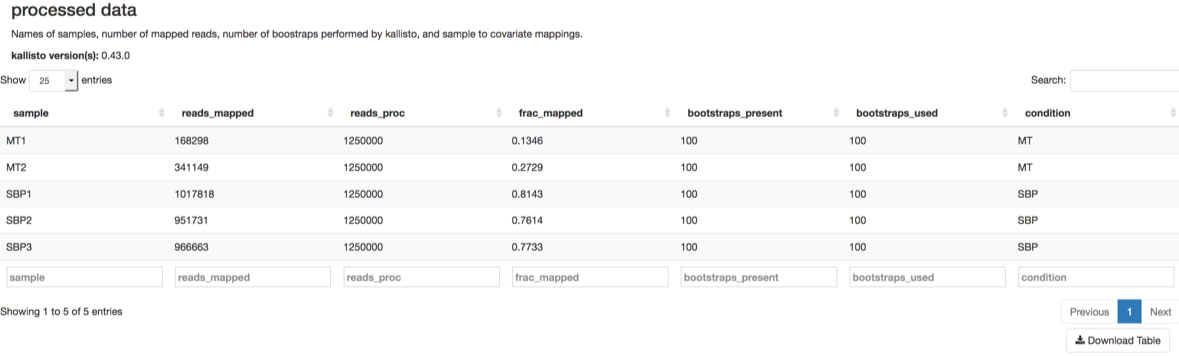
\includegraphics{images/sleuth-processed-data.png}
\caption{sleuth - processed data table}
\end{figure}

    In some cases, we can identify samples which don't agree with other
replicates (\textbf{outliers}) and samples which are related by
experimental bias (\textbf{batch effects}). If we don't have many
replicates, it's hard to detect outliers and batch effects meaning our
power to detect DE genes is reduced.

\textbf{Principal component analysis (PCA)} plots can be used to look at
variation and strong patterns within the dataset. Batch effects and
outliers often stand out quite clearly in the PCA plot and mean that you
can account for them in any downstream analysis.

    \begin{figure}[!h]
\centering
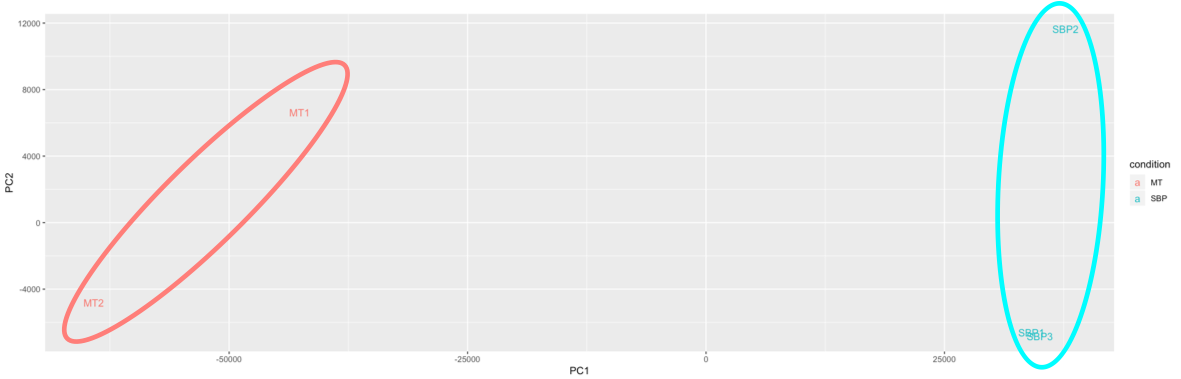
\includegraphics{images/sleuth-pca.png}
\caption{sleuth - PCA plot}
\end{figure}

\newpage

    Our samples form two condition-related clusters with the two MT samples
(red) on the left and the three SBP samples on the right (blue). If we
look at the variance bar plot, we can see that the first principal
component (PC1) accounts for \textgreater90\% of the variation in our
dataset. As the samples are clearly clustered on the x-axis (PC1) this
suggests that most of the variation in the dataset is related to our
experimental condition (Mt vs SBP).

    \begin{figure}[!h]
\centering
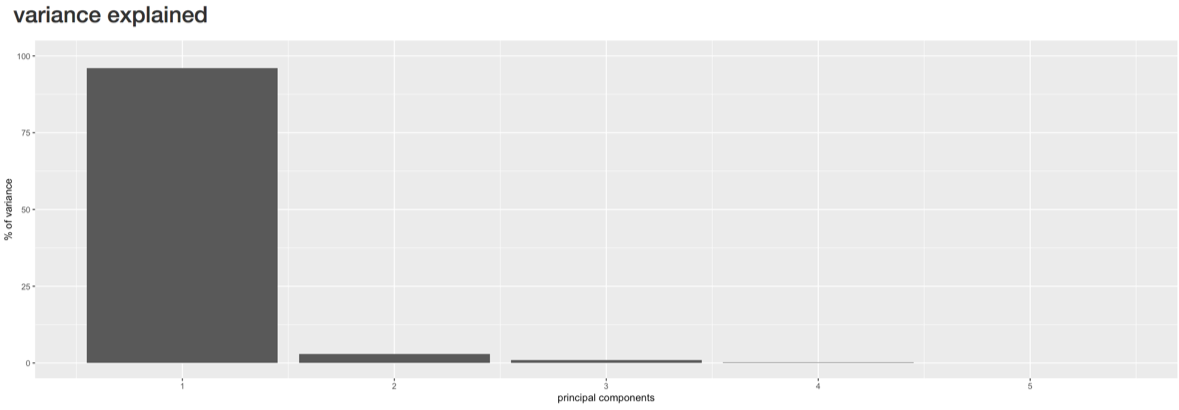
\includegraphics{images/sleuth-pca-bar.png}
\caption{sleuth - variance bar plot}
\end{figure}

    \hypertarget{using-sleuth-to-look-at-de-transcripts}{%
\subsubsection{Using sleuth to look at DE
transcripts}\label{using-sleuth-to-look-at-de-transcripts}}

We used the output from Kallisto to identify DE transcripts using
sleuth. Let's take a look and see if we found any.

\textbf{To see the results of the sleuth DEA, go to ``\textit{analyses
-\textgreater{} test table}''.}

    \begin{figure}[!h]
\centering
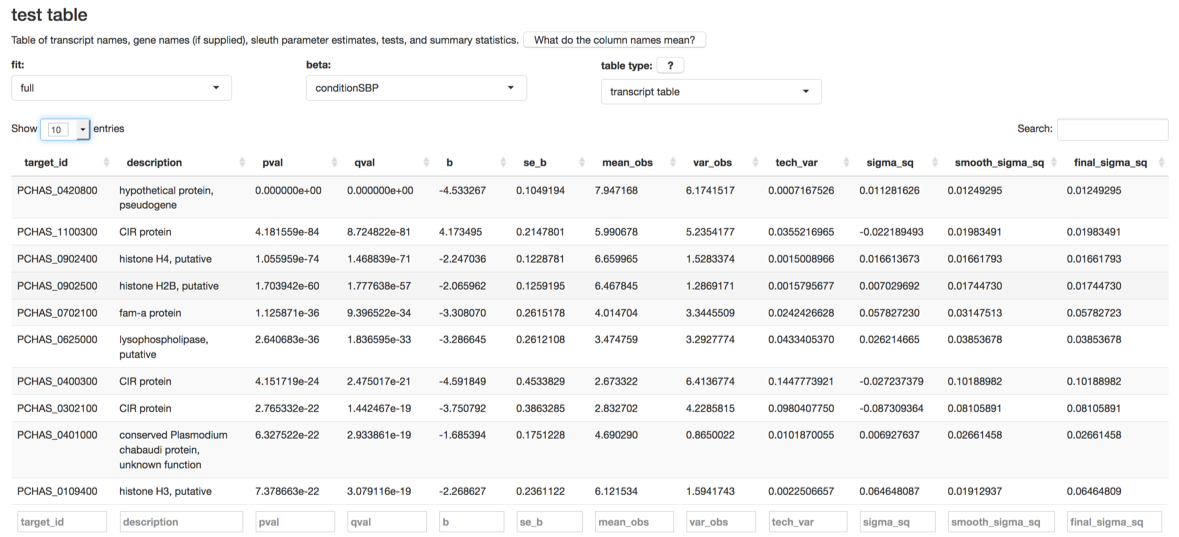
\includegraphics{images/sleuth-transcript-table.png}
\caption{sleuth - transcript table}
\end{figure}

    The important columns here are the \textbf{q-value} and the \textbf{beta
value} (analagous to fold change). By default, the table is sorted by
the q-value. We can see that our top transcript is PCHAS\_0420800, a
hypothetical protein/pseudogene. Now let's take a closer look at that
transcript.

\newpage

\textbf{Go to ``\textit{analyses -\textgreater{} transcript view}''. Enter
``PCHAS\_0420800'' into the ``\textit{transcript}'' search box. Click
``\textit{view}''.}

    \begin{figure}[!h]
\centering
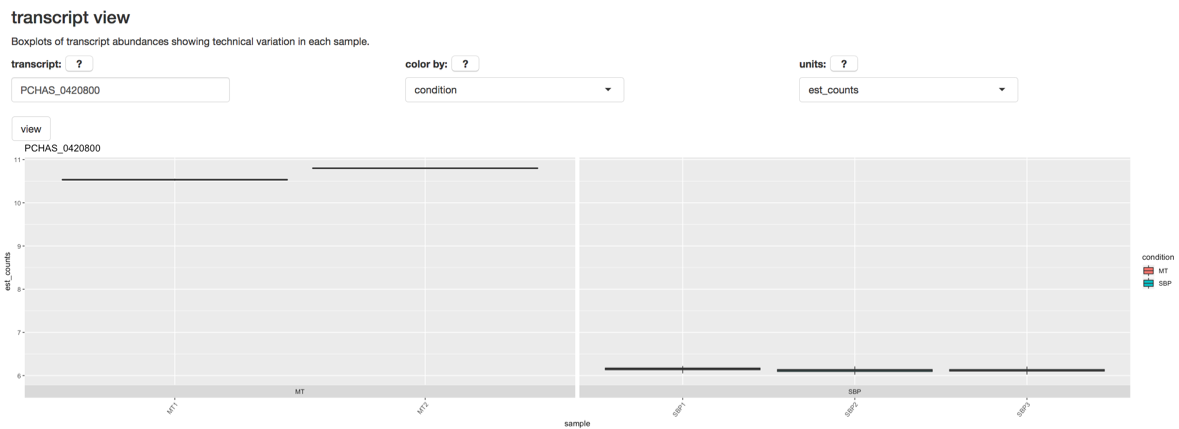
\includegraphics{images/sleuth-transcript-view.png}
\caption{sleuth - transcript view}
\end{figure}

    On the left you have the abundances for the MT replicates and on the
right, the SBP replicates. We can see that this transcript is more
highly expressed in the MT samples than in the SBP samples. This is also
reflected by the fold change in the test table (b = -4.5). The b value
is negative as it represents the fold change in SBP samples relative to
those in the MT samples.

Finally, let's take a look at the gene level.

\textbf{To see the results of the sleuth DEA, go to ``\textit{analyses
-\textgreater{} test\_table}''. Under ``\textit{table type}'' select
``\textit{gene table}''. Click on the column header ``\textit{qval}'' in the
table to sort the rows by ascending q-value.}

    \begin{figure}[!h]
\centering
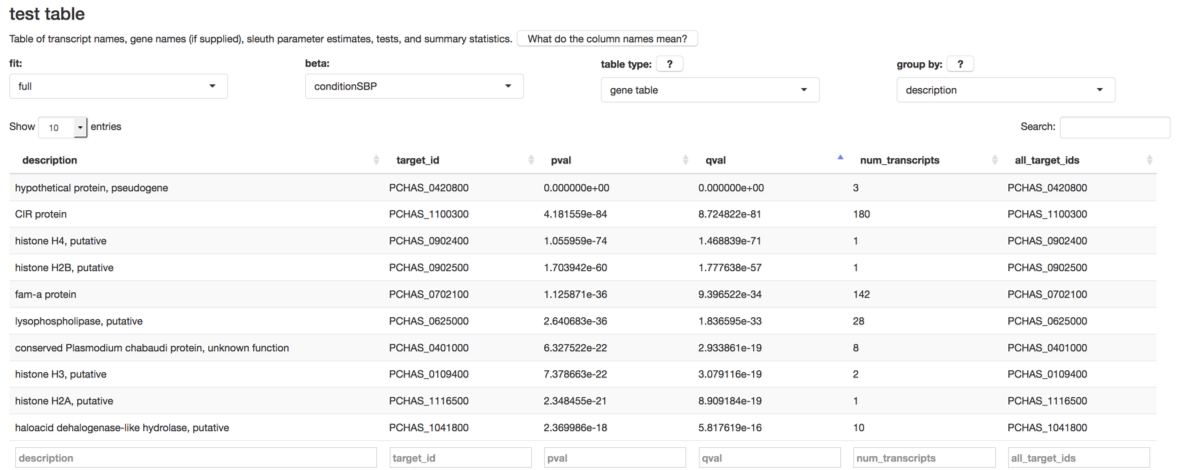
\includegraphics{images/sleuth-gene-table.png}
\caption{sleuth - gene table}
\end{figure}

    The transcripts have now been grouped by their descriptions. Let's take
a closer look at the CIR proteins.

\newpage

\textbf{Go to ``\textit{analyses -\textgreater{} gene view}''. In the
``\textit{gene}'' search box enter ``CIR protein'' (without the quotes).}

    \begin{figure}[!h]
\centering
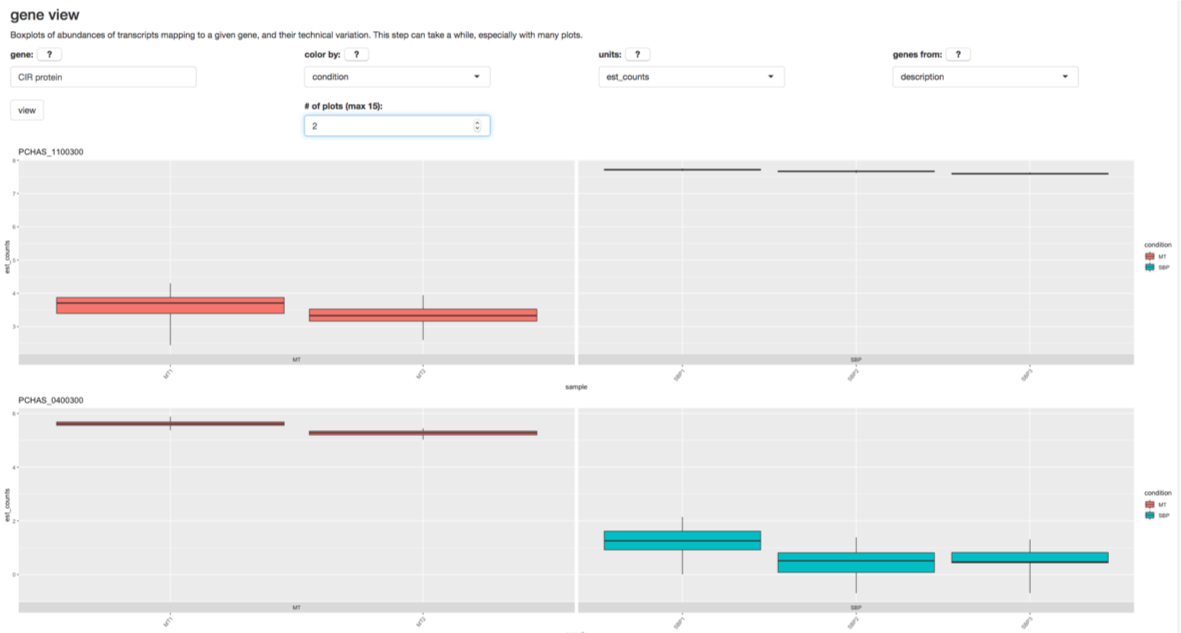
\includegraphics{images/sleuth-gene-view.png}
\caption{sleuth - gene view}
\end{figure}

    Here we can see the individual CIR protein transcript abundances. We can
see that PCHAS\_1100300 is more highly expressed in the SBP samples
while PCHAS\_0302100 and PCHAS\_0302100 are more highly expressed in the
MT samples.

    \begin{center}\rule{0.5\linewidth}{0.5pt}\end{center}

    \hypertarget{questions}{%
\subsection{Questions}\label{questions}}

\hypertarget{q1-is-our-gene-from-earlier-pchas_1402500-significantly-differentially-expressed}{%
\subsubsection{Q1: Is our gene from earlier, PCHAS\_1402500,
significantly differentially
expressed?}\label{q1-is-our-gene-from-earlier-pchas_1402500-significantly-differentially-expressed}}


    % Add a bibliography block to the postdoc



\newpage





    \hypertarget{interpreting-the-results}{%
\section{Interpreting the results}\label{interpreting-the-results}}

    \hypertarget{introduction}{%
\subsection{Introduction}\label{introduction}}

The main objective of this part of the tutorial is to use simple Unix
commands to get a list of significantly differentially expressed genes.
Using this gene list and the quantitative information from our analysis
we can then start to make biological inferences about our dataset.

Using the R script (\texttt{sleuth.R}), we printed out a file of results
describing the differentially expressed genes in our dataset. This file
is called \textbf{\texttt{kallisto.results}}.

The file contains several columns, of which the most important are:

\begin{itemize}
\tightlist
\item
  \textbf{Column 1}: target\_id (gene id)\\
\item
  \textbf{Column 2}: description (some more useful description of the
  gene than its id)\\
\item
  \textbf{Column 3}: pval (p value)\\
\item
  \textbf{Column 4}: qval (p value corrected for multiple hypothesis
  testing)\\
\item
  \textbf{Column 5}: b (fold change)
\end{itemize}

With a little Linux magic we can get the list of differentially
expressed genes with only the columns of interest as above.

    \begin{center}\rule{0.5\linewidth}{0.5pt}\end{center}

    \#\#~Exercise 6

    To get the genes which are most highly expressed in our SBP samples, we
must first filter our results. There are two columns we want to filter
our data on: \textbf{b} (column 5) and \textbf{qval} (column 4). These
columns represent whether the gene is differentially expressed and
whether that change is significant.

The following command will get those genes which have an adjusted p
value (qval) less than 0.01 and a positive fold change. These genes are
more highly expressed in the SBP samples.

    \begin{tcolorbox}[breakable, size=fbox, boxrule=1pt, pad at break*=1mm,colback=cellbackground, colframe=cellborder]
\prompt{In}{incolor}{ }{\boxspacing}
\begin{Verbatim}[commandchars=\\\{\}]
awk \PYZhy{}F \PY{l+s+s2}{\PYZdq{}\PYZbs{}t\PYZdq{}} \PY{l+s+s1}{\PYZsq{}\PYZdl{}4 \PYZlt{} 0.01 \PYZam{}\PYZam{} \PYZdl{}5 \PYZgt{} 0\PYZsq{}} data/kallisto.results \PY{p}{|} cut \PYZhy{}f1,2,3,4,5 \PY{p}{|} head
\end{Verbatim}
\end{tcolorbox}

    We used \texttt{awk} to filter the gene list and print only the lines
which met our search criteria (qval \textgreater{} 0.01, b
\textgreater{} 0). The option \texttt{-F} tells awk what delimiter is
used to separate the columns. In this case, it was a tab or its regular
expression "\t". We then use cut to only print out columns 1-5. You can
also do that within the \texttt{awk} command. Finally, we use
\texttt{head} to get the first 10 lines of the output.

Alternatively, we can look for the genes which are more highly expressed
in the MT samples.

    \begin{tcolorbox}[breakable, size=fbox, boxrule=1pt, pad at break*=1mm,colback=cellbackground, colframe=cellborder]
\prompt{In}{incolor}{ }{\boxspacing}
\begin{Verbatim}[commandchars=\\\{\}]
awk \PYZhy{}F \PY{l+s+s2}{\PYZdq{}\PYZbs{}t\PYZdq{}} \PY{l+s+s1}{\PYZsq{}\PYZdl{}4 \PYZlt{} 0.01 \PYZam{}\PYZam{} \PYZdl{}5 \PYZlt{} 0\PYZsq{}} data/kallisto.results \PY{p}{|} cut \PYZhy{}f1,2,3,4,5 \PY{p}{|} head
\end{Verbatim}
\end{tcolorbox}

    It can be useful to have a quick look and compare gene lists. For
example, whether a certain gene product is seen more often in the genes
most highly expressed in one condition or another. A quick and dirty
method would be to use the gene descriptions (or gene products).

You could extract the gene products (column 2) for genes which are more
highly expressed in the SBP samples using \texttt{sort} and then
\texttt{uniq}.

    \begin{tcolorbox}[breakable, size=fbox, boxrule=1pt, pad at break*=1mm,colback=cellbackground, colframe=cellborder]
\prompt{In}{incolor}{ }{\boxspacing}
\begin{Verbatim}[commandchars=\\\{\}]
awk \PYZhy{}F \PY{l+s+s2}{\PYZdq{}\PYZbs{}t\PYZdq{}} \PY{l+s+s1}{\PYZsq{}\PYZdl{}4 \PYZlt{} 0.01 \PYZam{}\PYZam{} \PYZdl{}5 \PYZlt{} 0 \PYZob{}print \PYZdl{}2\PYZcb{}\PYZsq{}} data/kallisto.results \PY{p}{|} sort \PY{p}{|} uniq
\end{Verbatim}
\end{tcolorbox}

    We can count each time these unique gene products occur in the list
using \texttt{uniq\ -c}.

    \begin{tcolorbox}[breakable, size=fbox, boxrule=1pt, pad at break*=1mm,colback=cellbackground, colframe=cellborder]
\prompt{In}{incolor}{ }{\boxspacing}
\begin{Verbatim}[commandchars=\\\{\}]
awk \PYZhy{}F \PY{l+s+s2}{\PYZdq{}\PYZbs{}t\PYZdq{}} \PY{l+s+s1}{\PYZsq{}\PYZdl{}4 \PYZlt{} 0.01 \PYZam{}\PYZam{} \PYZdl{}5 \PYZlt{} 0 \PYZob{}print \PYZdl{}2\PYZcb{}\PYZsq{}} data/kallisto.results \PY{p}{|} \PY{l+s+se}{\PYZbs{}}
sort \PY{p}{|} uniq \PYZhy{}c
\end{Verbatim}
\end{tcolorbox}

    And, if we wanted to make it a bit easier to see commonly found gene
products we can sort this again by the frequency count we got from the
\texttt{uniq} command. The \texttt{sort} command will put these in
ascending numerical (-n) order.

    \begin{tcolorbox}[breakable, size=fbox, boxrule=1pt, pad at break*=1mm,colback=cellbackground, colframe=cellborder]
\prompt{In}{incolor}{ }{\boxspacing}
\begin{Verbatim}[commandchars=\\\{\}]
awk \PYZhy{}F \PY{l+s+s2}{\PYZdq{}\PYZbs{}t\PYZdq{}} \PY{l+s+s1}{\PYZsq{}\PYZdl{}4 \PYZlt{} 0.01 \PYZam{}\PYZam{} \PYZdl{}5 \PYZlt{} 0 \PYZob{}print \PYZdl{}2\PYZcb{}\PYZsq{}} data/kallisto.results \PY{p}{|} \PY{l+s+se}{\PYZbs{}}
sort \PY{p}{|} uniq \PYZhy{}c \PY{p}{|} sort \PYZhy{}n
\end{Verbatim}
\end{tcolorbox}

    If you wanted to look for the frequency of a particular gene product you
could also use \texttt{grep}.

    \begin{tcolorbox}[breakable, size=fbox, boxrule=1pt, pad at break*=1mm,colback=cellbackground, colframe=cellborder]
\prompt{In}{incolor}{ }{\boxspacing}
\begin{Verbatim}[commandchars=\\\{\}]
awk \PYZhy{}F \PY{l+s+s2}{\PYZdq{}\PYZbs{}t\PYZdq{}} \PY{l+s+s1}{\PYZsq{}\PYZdl{}4 \PYZlt{} 0.01 \PYZam{}\PYZam{} \PYZdl{}5 \PYZlt{} 0 \PYZob{}print \PYZdl{}2\PYZcb{}\PYZsq{}} data/kallisto.results \PY{p}{|} grep \PYZhy{}c CIR
\end{Verbatim}
\end{tcolorbox}

    Or building on the earlier command:

    \begin{tcolorbox}[breakable, size=fbox, boxrule=1pt, pad at break*=1mm,colback=cellbackground, colframe=cellborder]
\prompt{In}{incolor}{ }{\boxspacing}
\begin{Verbatim}[commandchars=\\\{\}]
awk \PYZhy{}F \PY{l+s+s2}{\PYZdq{}\PYZbs{}t\PYZdq{}} \PY{l+s+s1}{\PYZsq{}\PYZdl{}4 \PYZlt{} 0.01 \PYZam{}\PYZam{} \PYZdl{}5 \PYZlt{} 0 \PYZob{}print \PYZdl{}2\PYZcb{}\PYZsq{}} data/kallisto.results \PY{p}{|} \PY{l+s+se}{\PYZbs{}}
sort \PY{p}{|} uniq \PYZhy{}c \PY{p}{|} grep CIR
\end{Verbatim}
\end{tcolorbox}

    If you want to read more about this work related to this data it is
published:

\begin{quote}
\textbf{Vector transmission regulates immune control of
\textit{Plasmodium} virulence}\\
Philip J. Spence, William Jarra, Prisca Lévy, Adam J. Reid, Lia
Chappell, Thibaut Brugat, Mandy Sanders, Matthew Berriman and Jean
Langhorne\\
\textit{Nature. 2013 Jun 13; 498(7453): 228--231
doi:\href{https://www.nature.com/articles/nature12231}{10.1038/nature12231}}
\end{quote}

    \begin{center}\rule{0.5\linewidth}{0.5pt}\end{center}

    \hypertarget{questions}{%
\subsection{Questions}\label{questions}}

    \hypertarget{q1-how-many-genes-are-more-highly-expressed-in-the-sbp-samples}{%
\subsubsection{Q1: How many genes are more highly expressed in the SBP
samples?}\label{q1-how-many-genes-are-more-highly-expressed-in-the-sbp-samples}}

\textit{Hint: try replacing \texttt{head} in the earlier command with
another unix command to count the number of lines}

\hypertarget{q2-how-many-genes-are-more-highly-expressed-in-the-mt-samples}{%
\subsubsection{Q2: How many genes are more highly expressed in the MT
samples?}\label{q2-how-many-genes-are-more-highly-expressed-in-the-mt-samples}}

\textit{Hint: try replacing \texttt{head} in the earlier command with
another unix command to count the number of lines}

\hypertarget{q3-do-you-notice-any-particular-genes-that-came-up-in-the-analysis}{%
\subsubsection{Q3: Do you notice any particular genes that came up in
the
analysis?}\label{q3-do-you-notice-any-particular-genes-that-came-up-in-the-analysis}}

\textit{Hint: look for gene products that are seen more often in genes
more highly expressed in the SBP samples than those more highly
expressed in the MT samples}

    % Add a bibliography block to the postdoc



\newpage





    \hypertarget{key-aspects-of-differential-expression-analysis}{%
\section{Key aspects of differential expression
analysis}\label{key-aspects-of-differential-expression-analysis}}

    \hypertarget{replicates-and-power}{%
\subsection{Replicates and power}\label{replicates-and-power}}

In order to accurately ascertain which genes are differentially
expressed and by how much it is necessary to use replicated data. As
with all biological experiments doing it once is simply not enough.
There is no simple way to decide how many replicates to do, it is
usually a compromise of statistical power and cost. By determining how
much variability there is in the sample preparation and sequencing
reactions, we can better assess how highly genes are really expressed
and more accurately determine any differences. The key to this is
performing biological rather than technical replicates. This means, for
instance, growing up three batches of parasites, treating them all
identically, extracting RNA from each and sequencing the three samples
separately. Technical replicates, whereby the same sample is sequenced
three times do not account for the variability that really exists in
biological systems or the experimental error between batches of
parasites and RNA extractions.

\textit{Note: more replicates will help improve power for genes that are
already detected at high levels, while deeper sequencing will improve
power to detect differential expression for genes which are expressed at
low levels.}

\hypertarget{p-values-vs.-q-values}{%
\subsection{p-values vs.~q-values}\label{p-values-vs.-q-values}}

When asking whether a gene is differentially expressed we use
statistical tests to assign a \textbf{p-value}. If a gene has a p-value
of 0.05, we say that there is only a 5\% chance that it is not really
differentially expressed. However, if we are asking this question for
every gene in the genome (\textasciitilde5500 genes for
\textit{Plasmodium}), then we would expect to see p-values less than 0.05
for many genes even though they are not really differentially expressed.
Due to this statistical problem, we must correct the p-values so that we
are not tricked into accepting a large number of erroneous results.
\textbf{Q-values} are p-values which have been corrected for what is
known as multiple hypothesis testing. Therefore, it is a q-value of less
than 0.05 that we should be looking for when asking whether a gene is
differentially expressed.

\hypertarget{alternative-software}{%
\subsection{Alternative software}\label{alternative-software}}

If you have a good quality genome and genome annotation such as for
model organisms e.g.~human, mouse, \textit{Plasmodium}; map to the
transcriptome to determine transcript abundance. This is even more
relevant if you have variant transcripts per gene as you need a tool
which will do its best to determine which transcript is really
expressed. As well as
\href{https://pachterlab.github.io/kallisto/}{Kallisto} (Bray et
al.~2016; PMID:
\href{https://www.ncbi.nlm.nih.gov/pubmed/27043002}{27043002}), there is
\href{https://pachterlab.github.io/eXpress/overview.html}{eXpress}
(Roberts \& Pachter, 2012; PMID:
\href{https://www.ncbi.nlm.nih.gov/pubmed/23160280}{23160280}) which
will do this.

Alternatively, you can map to the genome and then call abundance of
genes, essentially ignoring variant transcripts. This is more
appropriate where you are less confident about the genome annotation
and/or you don't have variant transcripts because your organism rarely
makes them or they are simply not annotated.
\href{https://ccb.jhu.edu/software/tophat/index.shtml}{Tophat2} (Kim et
al., 2013; PMID:
\href{https://www.ncbi.nlm.nih.gov/pubmed/23618408}{23618408}),
\href{https://ccb.jhu.edu/software/hisat2/index.shtml}{HISAT2} (Pertea
et al.~2016; PMID:
\href{https://www.ncbi.nlm.nih.gov/pubmed/27560171}{27560171}),
\href{https://github.com/alexdobin/STAR}{STAR} (Dobinet al., 2013; PMID:
\href{https://www.ncbi.nlm.nih.gov/pubmed/23104886}{23104886}) and
\href{http://research-pub.gene.com/gmap/}{GSNAP} (Wu \& Nacu, 2010;
PMID: \href{https://www.ncbi.nlm.nih.gov/pubmed/20147302}{20147302}) are
all splice-aware RNA-seq read mappers appropriate for this task. You
then need to use a tool which counts the reads overlapping each gene
model. \href{https://htseq.readthedocs.io/en/release_0.10.0/}{HTSeq}
(Anders et al., 2015; PMID:
\href{https://www.ncbi.nlm.nih.gov/pubmed/25260700}{25260700}) is a
popular tool for this purpose.
\href{https://github.com/cole-trapnell-lab/cufflinks}{Cufflinks}
(Trapnell et al.~2012; PMID:
\href{https://www.ncbi.nlm.nih.gov/pubmed/22383036}{22383036}) will
count reads and determine differentially expressed genes.

There are a variety of programs for detecting differentially expressed
genes from tables of RNA-seq read counts.
\href{https://bioconductor.org/packages/release/bioc/html/DESeq2.html}{DESeq2}
(Love et al., 2014; PMID:
\href{https://www.ncbi.nlm.nih.gov/pubmed/25516281}{25516281}),
\href{https://bioconductor.org/packages/release/bioc/html/edgeR.html}{EdgeR}
(Robinson et al., 2010; PMID:
\href{https://www.ncbi.nlm.nih.gov/pubmed/19910308}{19910308}) and
\href{http://bioconductor.org/packages/release/bioc/html/baySeq.html}{BaySeq}
(Hardcastle \& Kelly, 2010; PMID:
\href{https://www.ncbi.nlm.nih.gov/pubmed/20698981}{20698981}) are good
examples.

\hypertarget{what-do-i-do-with-a-gene-list}{%
\subsection{What do I do with a gene
list?}\label{what-do-i-do-with-a-gene-list}}

Differential expression analysis results are a list of genes which show
differences between two conditions. It can be daunting trying to
determine what the results mean. On one hand, you may find that that
there are no real differences in your experiment. Is this due to
biological reality or noisy data? On the other hand, you may find
several thousands of genes are differentially expressed. What can you
say about that?

Other than looking for genes you expect to be different or unchanged,
one of the first things to do is look at \textbf{Gene Ontology (GO) term
enrichment}. There are many different algorithms for this, but you could
annotate your genes with functional terms from GO using for instance
\url{Blast2GO} (Conesa et al., 2005; PMID:
\href{https://www.ncbi.nlm.nih.gov/pubmed/16081474}{16081474}) and then
use
\href{https://bioconductor.org/packages/release/bioc/html/topGO.html}{TopGO}
(Alexa et al., 2005; PMID:
\href{https://www.ncbi.nlm.nih.gov/pubmed/16606683}{16606683}) to
determine whether any particular sorts of genes occur more than expected
in your differentially expressed genes.

    \begin{center}\rule{0.5\linewidth}{0.5pt}\end{center}

    \hypertarget{congratulations-you-have-reached-the-end-of-this-tutorial}{%
\subsection{Congratulations, you have reached the end of this
tutorial!}\label{congratulations-you-have-reached-the-end-of-this-tutorial}}

We hope you've enjoyed our RNA-Seq tutorial!


    % Add a bibliography block to the postdoc



\newpage





    \hypertarget{normalisation}{%
\section{Normalisation}\label{normalisation}}

\hypertarget{introduction}{%
\subsection{Introduction}\label{introduction}}

In the previous section, we looked at estimating transcript abundance
with Kallisto. The abundances are reported as \textbf{transcripts per
million (TPM)}, but what does TPM mean and how is it calculated?

The objectives of this part of the tutorial are:

\begin{itemize}
\tightlist
\item
  \textit{understand why RNA-Seq normalisation metrics are used}
\item
  \textit{understand the difference between RPKM, FPKM and TPM}
\item
  \textit{calculate RPKM and TPM for a gene of interest}
\end{itemize}

There are many useful websites, publications and blog posts which go
into much more detail about RNA-Seq normalisation methods. Here are just
a couple (in no particular order):

\begin{itemize}
\tightlist
\item
  \href{https://haroldpimentel.wordpress.com/2014/05/08/what-the-fpkm-a-review-rna-seq-expression-units/}{What
  the FPKM? A review of RNA-Seq expression units}
\item
  \href{https://statquest.org/2015/07/09/rpkm-fpkm-and-tpm-clearly-explained/}{RPKM,
  FPKM and TPM, clearly explained}
\item
  \href{https://www.ncbi.nlm.nih.gov/pmc/articles/PMC4728800/}{A survey
  of best practices for RNA-seq data analysis}
\item
  \href{http://robpatro.com/blog/?p=235}{The RNA-seq abundance zoo}
\end{itemize}

    \hypertarget{why-do-we-use-normalisation-units-instead-of-raw-counts}{%
\subsection{Why do we use normalisation units instead of raw
counts?}\label{why-do-we-use-normalisation-units-instead-of-raw-counts}}

Raw reads counts are the number of reads originating from each
transcript which can be affected by several factors:

\begin{itemize}
\item
  \textbf{sequencing depth (total number of reads)}\\
  The more we sequence a sample, the more reads we expect to be
  assigned.
\item
  \textbf{gene/transcript length}\\
  The longer the gene or transcript, the more reads we expect to be
  assigned to it.
\end{itemize}

    \begin{figure}[!h]
\centering
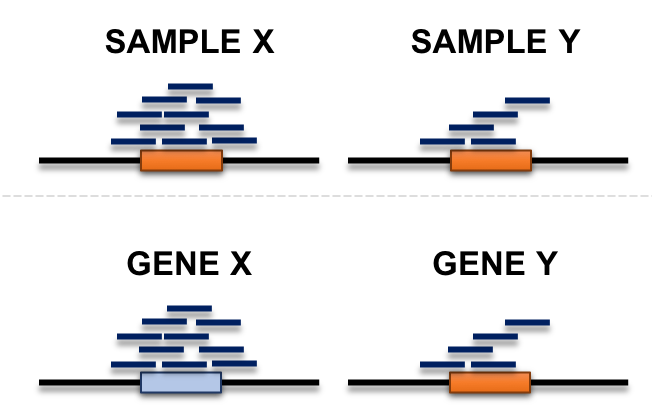
\includegraphics{images/count-bias.png}
\caption{Figure 4. Effect of sequencing depth and gene length on raw
read counts}
\end{figure}

\newpage

    \textit{Look at the top part of Figure 4. In which sample, X or Y, is the
gene more highly expressed?}

Neither, it's the same in both. What we didn't tell you was that the
total number of reads generated for sample A was twice the number than
for sample B. That meant almost twice the number of reads are assigned
to the same gene in sample A than in sample B.

\textit{Look at the bottom part of Figure 4. Which gene, X or Y, has the
greatest gene level expression?}

Neither, they are both expressed at the same level. This time we didn't
tell you that gene X is twice the length of gene Y. This meant that
almost twice the number reads were assigned to gene X than gene Y.

In the top part of \textit{Figure 4}, the gene in sample X has twice the
number of reads assigned to it than the same gene in sample Y. What
isn't shown is that sample X had twice the number or total reads than
sample Y so we would expect more reads to be assigned in sample X. Thus,
the gene is expressed at roughly the same level in both samples. In the
bottom part of \textit{Figure 4}, gene X has twice the number of reads
assigned to it than gene Y. However, gene X is twice the length of gene
Y and so we expect more reads to be assigned to gene X. Again, the
expression level is roughly the same.

    \hypertarget{reads-per-kilobase-per-million-rpkm}{%
\subsubsection{Reads per kilobase per million
(RPKM)}\label{reads-per-kilobase-per-million-rpkm}}

Reads per kilobase (of exon) per million (reads mapped) or \textbf{RPKM}
is a \textbf{within sample} normalisation method which takes into
account sequencing depth and length biases.

To calculate RPKM, you first normalise by sequencing depth and then by
gene/transcript length.

\begin{enumerate}
\def\labelenumi{\arabic{enumi}.}
\item
  \textbf{Get your \textit{per million} scaling factor}\\
  Count up the total number of reads which have been assigned (mapped)
  in the sample. Divide this number by 1,000,000 (1 million) to get your
  \textit{per million} scaling factor (N).
\item
  \textbf{Normalise for sequencing depth}\\
  Divide the number of reads which have been assigned to the gene or
  transcript (C) by the \textit{per million} scaling factor you calculated
  in step 1. This will give you your reads per million (RPM).
\item
  \textbf{Get your \textit{per kilobase} scaling factor}\\
  Divide the total length of the exons in your transcript or gene in
  base pairs by 1,000 (1 thousand) to get your \textit{per kilobase}
  scaling factor (L).
\item
  \textbf{Normalise for length}\\
  Divide your RPM value from step 2 by your \textit{per kilobase} scaling
  factor (length of the gene/transcript in kilobases) from step 3. This
  will give you your reads per kilobase per million or RPKM.
\end{enumerate}

This can be simplified into the following equation:

\begin{equation*}
RPKM = \frac {C}{LN}
\end{equation*}

\newpage

Where:

\begin{itemize}
\tightlist
\item
  \textbf{C} is number of reads mapped to the transcript or gene
\item
  \textbf{L} is the total exon length of the transcript or gene in
  kilobases
\item
  \textbf{N} is the total number of reads mapped in millions
\end{itemize}

    \hypertarget{fragments-per-kilobase-per-million-fpkm}{%
\subsubsection{Fragments per kilobase per million
(FPKM)}\label{fragments-per-kilobase-per-million-fpkm}}

Fragments per kilobase per million or \textbf{FPKM} is essentially the
same as RPKM except that:

\begin{itemize}
\item
  RPKM is designed for \textbf{single-end} RNA-Seq experiments
\item
  FPKM is designed for \textbf{paired-end} RNA-Seq experiments
\end{itemize}

In a paired-end RNA-Seq experiment, two reads may be assigned to a
single fragment (in any orientation). Also, in some cases, only one of
those reads will be assigned to a fragment (singleton). The only
difference between RPKM and FPKM is that FPKM takes into consideration
that two reads may be assigned to the same fragment.

    \hypertarget{transcripts-per-million-tpm}{%
\subsubsection{Transcripts per million
(TPM)}\label{transcripts-per-million-tpm}}

Calculating the \textbf{transcripts per million} or \textbf{TPM} is a
similar process to RPKM and FPKM. The main difference is that you will
first normalise for length bias and then for sequencing depth bias. In a
nut shell, we are swapping the order of normalisations.

\begin{enumerate}
\def\labelenumi{\arabic{enumi}.}
\item
  \textbf{Get your \textit{per kilobase} scaling factor}\\
  Divide the total length of the exons in your transcript in base pairs
  by 1,000 (1 thousand) to get your \textit{per kilobase} scaling factor.
\item
  \textbf{Normalise for length}\\
  Divide the number of reads which have been assigned to the transcript
  by the per kilobase scaling factor you calculated in step 1. This will
  give you your reads per kilobase (RPK).
\item
  \textbf{Get the sum of all RPK values in your sample}\\
  Calculate the RPK value for all of the transcripts in your sample. Add
  all of these together to get your total RPK value.
\item
  \textbf{Get your \textit{per million} scaling factor}\\
  Divide your total RPK value from step 3 by 1,000,000 (1 million) to
  get your \textit{per million} scaling factor.
\item
  \textbf{Normalise for sequencing depth}\\
  Divide your RPK value calculated in step 2 by the \textit{per million}
  scaling factor from step 4. You now have your transcripts per millions
  value or TPM.
\end{enumerate}

\newpage

    \hypertarget{calculating-rpkm-and-tpm-values}{%
\subsection{Calculating RPKM and TPM
values}\label{calculating-rpkm-and-tpm-values}}

To try and answer this, let's look at a worked example. Here, we have
three genes (A-C) and three biological replicates (1-3).

\begin{longtable}[]{@{}ccccc@{}}
\toprule
Gene & Length & Replicate 1 & Replicate 2 & Replicate 3\tabularnewline
\midrule
\endhead
\textbf{A} & 2,000 bases & 10 & 12 & 30\tabularnewline
\textbf{B} & 4,000 bases & 20 & 25 & 60\tabularnewline
\textbf{C} & 1,000 bases & 5 & 8 & 15\tabularnewline
\bottomrule
\end{longtable}

There are two things to notice in our dataset:

\begin{itemize}
\item
  Gene B has twice number reads mapped than gene A, possibly as it's
  twice the length
\item
  Replicate 3 has more reads mapped than any of the other replicates,
  regardless of which gene we look at
\end{itemize}

\hypertarget{calculating-rpkm}{%
\subsubsection{Calculating RPKM}\label{calculating-rpkm}}

\hypertarget{step-1-get-your-per-million-scaling-factor}{%
\paragraph{Step 1: get your per million scaling
factor}\label{step-1-get-your-per-million-scaling-factor}}

In the table below is the total number of reads which mapped for each of
the replicates. To get our \textit{per million} scaling factor, we divide
each of these values by 1,000,000 (1 million).

\begin{longtable}[]{@{}cccc@{}}
\toprule
Gene & Replicate 1 & Replicate 2 & Replicate 3\tabularnewline
\midrule
\endhead
Total reads mapped & 3,500,000 & 4,500,000 & 10,600,000\tabularnewline
Per million reads & 3.5 & 4.5 & 10.6\tabularnewline
\bottomrule
\end{longtable}

\hypertarget{step-2-normalise-for-sequencing-depth}{%
\paragraph{Step 2: normalise for sequencing
depth}\label{step-2-normalise-for-sequencing-depth}}

We now divide our read counts by the \textit{per million} scaling factor
to get our reads per million (RPM).

Before:

\begin{longtable}[]{@{}cccc@{}}
\toprule
Gene & Replicate 1 & Replicate 2 & Replicate 3\tabularnewline
\midrule
\endhead
\textbf{A} & 10 & 12 & 30\tabularnewline
\textbf{B} & 20 & 25 & 60\tabularnewline
\textbf{C} & 5 & 8 & 15\tabularnewline
\bottomrule
\end{longtable}

\newpage

After:

\begin{longtable}[]{@{}cccc@{}}
\toprule
Gene & Replicate 1 RPM & Replicate 2 RPM & Replicate 3
RPM\tabularnewline
\midrule
\endhead
\textbf{A} & 2.857 & 2.667 & 2.830\tabularnewline
\textbf{B} & 5.714 & 5.556 & 5.660\tabularnewline
\textbf{C} & 1.429 & 1.778 & 1.415\tabularnewline
\bottomrule
\end{longtable}

\hypertarget{step-3-get-your-per-kilobase-scaling-factor}{%
\paragraph{\texorpdfstring{Step 3: get your \textit{per kilobase} scaling
factor}{Step 3: get your per kilobase scaling factor}}\label{step-3-get-your-per-kilobase-scaling-factor}}

Here we have our gene length in base pairs. For our \textit{per kilobase}
scaling factor we need to get our gene length in kilobases by dividing
it by 1,000.

\begin{longtable}[]{@{}ccc@{}}
\toprule
Gene & Length (base pairs) & Length (kilobases)\tabularnewline
\midrule
\endhead
\textbf{A} & 2,000 & 2\tabularnewline
\textbf{B} & 4,000 & 4\tabularnewline
\textbf{C} & 1,000 & 1\tabularnewline
\bottomrule
\end{longtable}

\hypertarget{step-4-normalise-for-length}{%
\paragraph{Step 4: normalise for
length}\label{step-4-normalise-for-length}}

Finally, we divide our RPM values from step 2 by our \textit{per kilobase}
scaling factor from step 3 to get our reads per kilobase per million
(RPKM).

Before:

\begin{longtable}[]{@{}cccc@{}}
\toprule
Gene & Replicate 1 RPM & Replicate 2 RPM & Replicate 3
RPM\tabularnewline
\midrule
\endhead
\textbf{A} & 2.857 & 2.667 & 2.830\tabularnewline
\textbf{B} & 5.714 & 5.556 & 5.660\tabularnewline
\textbf{C} & 1.429 & 1.778 & 1.415\tabularnewline
\bottomrule
\end{longtable}

After:

\begin{longtable}[]{@{}cccc@{}}
\toprule
Gene & Replicate 1 RPKM & Replicate 2 RPKM & Replicate 3
RPKM\tabularnewline
\midrule
\endhead
\textbf{A} & 1.43 & 1.33 & 1.42\tabularnewline
\textbf{B} & 1.43 & 1.39 & 1.42\tabularnewline
\textbf{C} & 1.43 & 1.78 & 1.42\tabularnewline
\bottomrule
\end{longtable}

Notice that even though replicate 3 had more reads assigned than the
other samples and a greater sequencing depth, its RPKM is quite similar.
And, that although gene B had twice the number of reads assigned than
gene A, its RPKM is the same. This is because we have normalised by both
length and sequencing depth.

    \hypertarget{calculating-tpm}{%
\subsubsection{Calculating TPM}\label{calculating-tpm}}

Now we're going to calculate the TPM values for the same example data.
As a reminder, here are our three genes (A-C) and three biological
replicates (1-3).

\begin{longtable}[]{@{}ccccc@{}}
\toprule
Gene & Length & Replicate 1 & Replicate 2 & Replicate 3\tabularnewline
\midrule
\endhead
\textbf{A} & 2,000 bases & 10 & 12 & 30\tabularnewline
\textbf{B} & 4,000 bases & 20 & 25 & 60\tabularnewline
\textbf{C} & 1,000 bases & 5 & 8 & 15\tabularnewline
\bottomrule
\end{longtable}

\hypertarget{step-1-get-your-per-kilobase-scaling-factor}{%
\paragraph{\texorpdfstring{Step 1: get your \textit{per kilobase} scaling
factor}{Step 1: get your per kilobase scaling factor}}\label{step-1-get-your-per-kilobase-scaling-factor}}

Again, our gene lengths are in base pairs. For our \textit{per kilobase}
scaling factor we need to get our gene length in kilobases by dividing
it by 1,000.

\begin{longtable}[]{@{}ccc@{}}
\toprule
Gene & Length (base pairs) & Length (kilobases)\tabularnewline
\midrule
\endhead
\textbf{A} & 2,000 & 2\tabularnewline
\textbf{B} & 4,000 & 4\tabularnewline
\textbf{C} & 1,000 & 1\tabularnewline
\bottomrule
\end{longtable}

\hypertarget{step-2-normalise-for-length}{%
\paragraph{Step 2: normalise for
length}\label{step-2-normalise-for-length}}

Now we divide the number of reads which have been assigned to each gene
by the per kilobase scaling factor we just calculated. This will give us
our reads per kilobase (RPK).

Before:

\begin{longtable}[]{@{}cccc@{}}
\toprule
Gene & Replicate 1 & Replicate 2 & Replicate 3\tabularnewline
\midrule
\endhead
\textbf{A} & 10 & 12 & 30\tabularnewline
\textbf{B} & 20 & 25 & 60\tabularnewline
\textbf{C} & 5 & 8 & 15\tabularnewline
\bottomrule
\end{longtable}

\newpage

After:

\begin{longtable}[]{@{}cccc@{}}
\toprule
Gene & Replicate 1 & Replicate 2 & Replicate 3\tabularnewline
\midrule
\endhead
\textbf{A} & 5 & 6 & 15\tabularnewline
\textbf{B} & 5 & 6.25 & 15\tabularnewline
\textbf{C} & 5 & 8 & 15\tabularnewline
\bottomrule
\end{longtable}

\hypertarget{step-3-get-the-sum-of-all-rpk-values-in-your-sample}{%
\paragraph{Step 3: get the sum of all RPK values in your
sample}\label{step-3-get-the-sum-of-all-rpk-values-in-your-sample}}

Next, we sum the RPK values for each of our replices. This will give use
our total RPK value for each replicate. To make this example scalable,
we assume there are other genes so the total RPK is made up.

\begin{longtable}[]{@{}cccc@{}}
\toprule
Gene & Replicate 1 & Replicate 2 & Replicate 3\tabularnewline
\midrule
\endhead
\textbf{A} & 5 & 6 & 15\tabularnewline
\textbf{B} & 5 & 6.25 & 15\tabularnewline
\textbf{C} & 5 & 8 & 15\tabularnewline
\ldots{} & \ldots{} & \ldots{} & \ldots{}\tabularnewline
\textbf{Total RPK} & \textbf{150,000} & \textbf{202,500} &
\textbf{450,000}\tabularnewline
\bottomrule
\end{longtable}

\hypertarget{step-4-get-your-per-million-scaling-factor}{%
\paragraph{\texorpdfstring{Step 4: get your \textit{per million} scaling
factor}{Step 4: get your per million scaling factor}}\label{step-4-get-your-per-million-scaling-factor}}

Here, instead of dividing our total mapped reads by 1,000,000 (1
million) to get our \textit{per million} scaling factor, we divide our
total RPK values by 1,000,000 (1 million).

\begin{longtable}[]{@{}cccc@{}}
\toprule
Gene & Replicate 1 & Replicate 2 & Replicate 3\tabularnewline
\midrule
\endhead
Total RPK & 150,000 & 202,500 & 450,000\tabularnewline
Per million RPK & 0.1500 & 0.2025 & 0.4500\tabularnewline
\bottomrule
\end{longtable}

\newpage

\hypertarget{step-5-normalise-for-sequencing-depth}{%
\paragraph{Step 5: normalise for sequencing
depth}\label{step-5-normalise-for-sequencing-depth}}

Finally, we divide our individual RPK values from step 2 by the
\textit{per million} scaling factor in step 4 to give us our TPM values.

Before:

\begin{longtable}[]{@{}cccc@{}}
\toprule
Gene & Replicate 1 & Replicate 2 & Replicate 3\tabularnewline
\midrule
\endhead
\textbf{A} & 5 & 6 & 15\tabularnewline
\textbf{B} & 5 & 6.25 & 15\tabularnewline
\textbf{C} & 5 & 8 & 15\tabularnewline
\bottomrule
\end{longtable}

After:

\begin{longtable}[]{@{}cccc@{}}
\toprule
Gene & Replicate 1 & Replicate 2 & Replicate 3\tabularnewline
\midrule
\endhead
\textbf{A} & 33.33 & 29.63 & 33.33\tabularnewline
\textbf{B} & 33.33 & 30.86 & 33.33\tabularnewline
\textbf{C} & 33.33 & 39.51 & 33.33\tabularnewline
\bottomrule
\end{longtable}

    \hypertarget{which-normalisation-unit-should-i-use}{%
\subsection{Which normalisation unit should I
use?}\label{which-normalisation-unit-should-i-use}}

Well, there's a lot of debate around this, so let's look at our total
normalised values for each replicate.

\hypertarget{rpkm}{%
\subsubsection{RPKM}\label{rpkm}}

\begin{longtable}[]{@{}cccc@{}}
\toprule
Gene & Replicate 1 RPKM & Replicate 2 RPKM & Replicate 3
RPKM\tabularnewline
\midrule
\endhead
\textbf{A} & 1.43 & 1.33 & 1.42\tabularnewline
\textbf{B} & 1.43 & 1.39 & 1.42\tabularnewline
\textbf{C} & 1.43 & 1.78 & 1.42\tabularnewline
\textbf{Total RPKM} & \textbf{4.29} & \textbf{4.50} &
\textbf{4.25}\tabularnewline
\bottomrule
\end{longtable}

\hypertarget{tpm}{%
\subsubsection{TPM}\label{tpm}}

\begin{longtable}[]{@{}cccc@{}}
\toprule
Gene & Replicate 1 & Replicate 2 & Replicate 3\tabularnewline
\midrule
\endhead
\textbf{A} & 33.33 & 29.63 & 33.33\tabularnewline
\textbf{B} & 33.33 & 30.86 & 33.33\tabularnewline
\textbf{C} & 33.33 & 39.51 & 33.33\tabularnewline
\textbf{Total TPM} & \textbf{100} & \textbf{100} &
\textbf{100}\tabularnewline
\bottomrule
\end{longtable}

Notice that that total TPM value for each of the replicates is the same.
This is not true for RPKM and FPKM where the total values differ. With
TPM, having the same total value for each replicate makes it easier to
compare the proportion of reads mapping to each gene across replicates
(although you shouldn't really compare across experiments). With RPKM
and FPKM, the differing total values make it much harder to compare
replicates.

    \begin{center}\rule{0.5\linewidth}{0.5pt}\end{center}

    \hypertarget{questions}{%
\subsection{Questions}\label{questions}}

Below is the information for each of the five samples. You will need
this information to answer the questions. We have put all of commands
used to get this information in the \href{aanswers.ipynb}{answers}.

\begin{longtable}[]{@{}ccccc@{}}
\toprule
Sample & Total mapped reads & Transcript length & Assigned reads & Total
RPK\tabularnewline
\midrule
\endhead
MT1 & 2,353,750 & 3,697 & 2,541 & 293,431\tabularnewline
MT2 & 2,292,271 & 3,709 & 3,392 & 675,190\tabularnewline
SBP1 & 2,329,235 & 3,699 & 14,605 & 1,719,970\tabularnewline
SBP2 & 2,187,718 & 3,696 & 17,302 & 1,429,540\tabularnewline
SBP3 & 2,163,979 & 3,699 & 14,646 & 1,561,310\tabularnewline
\bottomrule
\end{longtable}

\textit{Note: values have been rounded up to integers to make calculations
easier. Assigned reads are the est\_count from Kallisto for
PCHAS\_1402500. Transcript lengths are the est\_length from Kallisto for
PCHAS\_1402500.}

\newpage

\textbf{Q1: Using the \texttt{abundance.tsv} files generated by Kallisto
and the information above, calculate the RPKM for PCHAS\_1402500 in each
of our five samples.}

\begin{longtable}[]{@{}ccccc@{}}
\toprule
Sample & Per million scaling factor & RPM & Per kilobase scaling factor
& RPKM\tabularnewline
\midrule
\endhead
MT1 & & & &\tabularnewline
MT2 & & & &\tabularnewline
SBP1 & & & &\tabularnewline
SBP2 & & & &\tabularnewline
SBP3 & & & &\tabularnewline
\bottomrule
\end{longtable}

\textbf{Q2: Using the \texttt{abundance.tsv} files generated by Kallisto
and the information above, calculate the TPM for PCHAS\_1402500 in each
of our five samples.}\\
\textit{Hint: don't forget to get your per million scaling factor.}

\begin{longtable}[]{@{}cccc@{}}
\toprule
Sample & Per kilobase scaling factor & Reads per kilobase (RPK) &
TPM\tabularnewline
\midrule
\endhead
MT1 & & &\tabularnewline
MT2 & & &\tabularnewline
SBP1 & & &\tabularnewline
SBP2 & & &\tabularnewline
SBP3 & & &\tabularnewline
\bottomrule
\end{longtable}

\textbf{Q3: Do these match the TPM values from Kallisto?}\\
\textit{Hint: look at the \texttt{abundance.tsv} files for each of your
samples.}

\textbf{Q4: Do you think PCHAS\_1402500 is differentially expressed
between the MT and SBP samples?}

    % Add a bibliography block to the postdoc



\newpage





    \hypertarget{running-commands-on-multiple-samples}{%
\section{Running commands on multiple
samples}\label{running-commands-on-multiple-samples}}

    Now, fair warning, you're going to wish we'd told you this earlier on.
However, then you wouldn't have had the fun of running and updating each
of the previous commands, growling at typos and generally wishing that
you'd gone for that cup of coffee before starting this tutorial.

Here we go\ldots.we can use a \textbf{loop} to run the same commands for
multiple samples.

There's a great introduction to bash scripting and loops as part of our
\textbf{Unix module}. But let's take a look at how we could have
generated genome alignments for all of our samples using a single loop.

Whenever you write a loop, it's always a good idea to build it up slowly
to check that it's doing what you think.

    \begin{tcolorbox}[breakable, size=fbox, boxrule=1pt, pad at break*=1mm,colback=cellbackground, colframe=cellborder]
\prompt{In}{incolor}{ }{\boxspacing}
\begin{Verbatim}[commandchars=\\\{\}]
\PY{k}{for} r in data/*.fastq.gz
\PY{k}{do}
  \PY{n+nb}{echo} \PY{n+nv}{\PYZdl{}r}
\PY{k}{done}
\end{Verbatim}
\end{tcolorbox}

    This loop looks for all (*) files which end with ``.fastq.gz''. The for
loop then executes a sequence of commands for each file name that it
finds. In the first iteration its ``data/MT1\_1.fastq.gz'', then
``data/MT1\_2.fastq.gz'' and so on\ldots{} In each iteration, we
assigned each filename that it found to a variable called ``r''.

\texttt{for\ r\ in\ *.fastq.gz}

Then, to check we got what we expected, we printed what the variable
``r'' represented back to the terminal. Because we want to use the
variable (``r'') we created we need to use dollar (\$) symbol.

\texttt{echo\ \$r}

Now, if we left things as they are, we would be running the commands
twice for each sample. This is because we have two FASTQ files for each
sample i.e.~"\_1.fastq.gz" and "\_2.fastq.gz``. Let's change our loop so
that we only get the''\_1.fastq.gz" files.

    \begin{tcolorbox}[breakable, size=fbox, boxrule=1pt, pad at break*=1mm,colback=cellbackground, colframe=cellborder]
\prompt{In}{incolor}{ }{\boxspacing}
\begin{Verbatim}[commandchars=\\\{\}]
\PY{k}{for} r1 in data/*\PYZus{}1.fastq.gz
\PY{k}{do}
  \PY{n+nb}{echo} \PY{n+nv}{\PYZdl{}r1}
\PY{k}{done}
\end{Verbatim}
\end{tcolorbox}

    Great! Now, the only problem here is that we're going to want to use
both the "\_1.fastq.gz" and the "\_2.fastq.gz" files in our mapping. We
can get around this by removing the ``data/'' directory and
"\_1.fastq.gz" suffix from the filename to give us our sample name.

\texttt{sample=\$(basename\ \$r1)}
\texttt{sample=\$\{sample/\_1.fastq.gz/\}}

This will get the base filename (e.g.~``MT1\_1.fastq.gz'') and replace
the "\_1.fastq.gz" at the end of the filename we stored as ``r1'' with
nothing.

    We've added a little descriptive message so that when we run our loop we
know which iteration it's on and what it's doing. Let's try adding our
HISAT2 mapping command.

\textit{Note: we assume that the HISAT2 index has already been generated
as that's a command you'll only need to run once.}

    \begin{tcolorbox}[breakable, size=fbox, boxrule=1pt, pad at break*=1mm,colback=cellbackground, colframe=cellborder]
\prompt{In}{incolor}{ }{\boxspacing}
\begin{Verbatim}[commandchars=\\\{\}]
\PY{k}{for} r1 in data/*\PYZus{}1.fastq.gz
\PY{k}{do}
  \PY{n+nv}{sample}\PY{o}{=}\PY{k}{\PYZdl{}(}basename \PY{n+nv}{\PYZdl{}r1}\PY{k}{)}
  \PY{n+nv}{sample}\PY{o}{=}\PY{l+s+si}{\PYZdl{}\PYZob{}}\PY{n+nv}{sample}\PY{p}{/\PYZus{}1.fastq.gz/}\PY{l+s+si}{\PYZcb{}}
  \PY{n+nb}{echo} \PY{l+s+s2}{\PYZdq{}Processing sample: \PYZdq{}}\PY{n+nv}{\PYZdl{}sample}

  \PY{n+nb}{echo} \PY{l+s+s2}{\PYZdq{}Mapping sample: \PYZdq{}}\PY{n+nv}{\PYZdl{}sample}
  hisat2 \PYZhy{}\PYZhy{}max\PYZhy{}intronlen \PY{l+m}{10000} \PYZhy{}x data/PccAS\PYZus{}v3\PYZus{}hisat2.idx \PY{l+s+se}{\PYZbs{}}
  \PYZhy{}1 \PY{l+s+s2}{\PYZdq{}}\PY{l+s+s2}{data/}\PY{l+s+si}{\PYZdl{}\PYZob{}}\PY{n+nv}{sample}\PY{l+s+si}{\PYZcb{}}\PY{l+s+s2}{\PYZus{}1.fastq.gz}\PY{l+s+s2}{\PYZdq{}} \PYZhy{}2 \PY{l+s+s2}{\PYZdq{}}\PY{l+s+s2}{data/}\PY{l+s+si}{\PYZdl{}\PYZob{}}\PY{n+nv}{sample}\PY{l+s+si}{\PYZcb{}}\PY{l+s+s2}{\PYZus{}2.fastq.gz}\PY{l+s+s2}{\PYZdq{}} \PYZhy{}S \PY{l+s+s2}{\PYZdq{}}\PY{l+s+s2}{data/}\PY{l+s+si}{\PYZdl{}\PYZob{}}\PY{n+nv}{sample}\PY{l+s+si}{\PYZcb{}}\PY{l+s+s2}{.sam}\PY{l+s+s2}{\PYZdq{}}
\PY{k}{done}
\end{Verbatim}
\end{tcolorbox}

    Notice that because we're using a variable as part of the filename, we
need to write the filename in double quotes.

\texttt{data/\$\{sample\}\_1.fastq.gz}

    Now let's add in our \texttt{samtools} commands.

    \begin{tcolorbox}[breakable, size=fbox, boxrule=1pt, pad at break*=1mm,colback=cellbackground, colframe=cellborder]
\prompt{In}{incolor}{ }{\boxspacing}
\begin{Verbatim}[commandchars=\\\{\}]
\PY{k}{for} r1 in data/*\PYZus{}1.fastq.gz
\PY{k}{do}
  \PY{n+nv}{sample}\PY{o}{=}\PY{k}{\PYZdl{}(}basename \PY{n+nv}{\PYZdl{}r1}\PY{k}{)}
  \PY{n+nv}{sample}\PY{o}{=}\PY{l+s+si}{\PYZdl{}\PYZob{}}\PY{n+nv}{sample}\PY{p}{/\PYZus{}1.fastq.gz/}\PY{l+s+si}{\PYZcb{}}
  \PY{n+nb}{echo} \PY{l+s+s2}{\PYZdq{}Processing sample: \PYZdq{}}\PY{n+nv}{\PYZdl{}sample}

  \PY{n+nb}{echo} \PY{l+s+s2}{\PYZdq{}Mapping sample: \PYZdq{}}\PY{n+nv}{\PYZdl{}sample}
  hisat2 \PYZhy{}\PYZhy{}max\PYZhy{}intronlen \PY{l+m}{10000} \PYZhy{}x data/PccAS\PYZus{}v3\PYZus{}hisat2.idx \PY{l+s+se}{\PYZbs{}}
  \PYZhy{}1 \PY{l+s+s2}{\PYZdq{}}\PY{l+s+s2}{data/}\PY{l+s+si}{\PYZdl{}\PYZob{}}\PY{n+nv}{sample}\PY{l+s+si}{\PYZcb{}}\PY{l+s+s2}{\PYZus{}1.fastq.gz}\PY{l+s+s2}{\PYZdq{}} \PYZhy{}2 \PY{l+s+s2}{\PYZdq{}}\PY{l+s+s2}{data/}\PY{l+s+si}{\PYZdl{}\PYZob{}}\PY{n+nv}{sample}\PY{l+s+si}{\PYZcb{}}\PY{l+s+s2}{\PYZus{}2.fastq.gz}\PY{l+s+s2}{\PYZdq{}} \PYZhy{}S \PY{l+s+s2}{\PYZdq{}}\PY{l+s+s2}{data/}\PY{l+s+si}{\PYZdl{}\PYZob{}}\PY{n+nv}{sample}\PY{l+s+si}{\PYZcb{}}\PY{l+s+s2}{.sam}\PY{l+s+s2}{\PYZdq{}}

  \PY{n+nb}{echo} \PY{l+s+s2}{\PYZdq{}Converting SAM to BAM: \PYZdq{}}\PY{n+nv}{\PYZdl{}sample}
  samtools view \PYZhy{}b \PYZhy{}o \PY{l+s+s2}{\PYZdq{}}\PY{l+s+s2}{data/}\PY{l+s+si}{\PYZdl{}\PYZob{}}\PY{n+nv}{sample}\PY{l+s+si}{\PYZcb{}}\PY{l+s+s2}{.bam}\PY{l+s+s2}{\PYZdq{}} \PY{l+s+s2}{\PYZdq{}}\PY{l+s+s2}{data/}\PY{l+s+si}{\PYZdl{}\PYZob{}}\PY{n+nv}{sample}\PY{l+s+si}{\PYZcb{}}\PY{l+s+s2}{.sam}\PY{l+s+s2}{\PYZdq{}}

  \PY{n+nb}{echo} \PY{l+s+s2}{\PYZdq{}Sorting BAM: \PYZdq{}}\PY{n+nv}{\PYZdl{}sample}
  samtools sort \PYZhy{}o \PY{l+s+s2}{\PYZdq{}}\PY{l+s+s2}{data/}\PY{l+s+si}{\PYZdl{}\PYZob{}}\PY{n+nv}{sample}\PY{l+s+si}{\PYZcb{}}\PY{l+s+s2}{\PYZus{}sorted.bam}\PY{l+s+s2}{\PYZdq{}} \PY{l+s+s2}{\PYZdq{}}\PY{l+s+s2}{data/}\PY{l+s+si}{\PYZdl{}\PYZob{}}\PY{n+nv}{sample}\PY{l+s+si}{\PYZcb{}}\PY{l+s+s2}{.bam}\PY{l+s+s2}{\PYZdq{}}

  \PY{n+nb}{echo} \PY{l+s+s2}{\PYZdq{}Indexing BAM: \PYZdq{}}\PY{n+nv}{\PYZdl{}sample}
  samtools index \PY{l+s+s2}{\PYZdq{}}\PY{l+s+s2}{data/}\PY{l+s+si}{\PYZdl{}\PYZob{}}\PY{n+nv}{sample}\PY{l+s+si}{\PYZcb{}}\PY{l+s+s2}{\PYZus{}sorted.bam}\PY{l+s+s2}{\PYZdq{}}
\PY{k}{done}
\end{Verbatim}
\end{tcolorbox}

\newpage

    Finally, we don't really want to keep intermediate SAM and unsorted BAM
files if we don't have to. They just take up precious space. So, let's
make our samtools command a one-liner, passing the stdout from one
command to another.

    \begin{tcolorbox}[breakable, size=fbox, boxrule=1pt, pad at break*=1mm,colback=cellbackground, colframe=cellborder]
\prompt{In}{incolor}{ }{\boxspacing}
\begin{Verbatim}[commandchars=\\\{\}]
\PY{k}{for} r1 in data/*\PYZus{}1.fastq.gz
\PY{k}{do}
  \PY{n+nv}{sample}\PY{o}{=}\PY{k}{\PYZdl{}(}basename \PY{n+nv}{\PYZdl{}r1}\PY{k}{)}
  \PY{n+nv}{sample}\PY{o}{=}\PY{l+s+si}{\PYZdl{}\PYZob{}}\PY{n+nv}{sample}\PY{p}{/\PYZus{}1.fastq.gz/}\PY{l+s+si}{\PYZcb{}}
  \PY{n+nb}{echo} \PY{l+s+s2}{\PYZdq{}Processing sample: \PYZdq{}}\PY{n+nv}{\PYZdl{}sample}
  hisat2 \PYZhy{}\PYZhy{}max\PYZhy{}intronlen \PY{l+m}{10000} \PYZhy{}x data/PccAS\PYZus{}v3\PYZus{}hisat2.idx \PY{l+s+se}{\PYZbs{}}
  \PYZhy{}1 \PY{l+s+s2}{\PYZdq{}}\PY{l+s+s2}{data/}\PY{l+s+si}{\PYZdl{}\PYZob{}}\PY{n+nv}{sample}\PY{l+s+si}{\PYZcb{}}\PY{l+s+s2}{\PYZus{}1.fastq.gz}\PY{l+s+s2}{\PYZdq{}} \PYZhy{}2 \PY{l+s+s2}{\PYZdq{}}\PY{l+s+s2}{data/}\PY{l+s+si}{\PYZdl{}\PYZob{}}\PY{n+nv}{sample}\PY{l+s+si}{\PYZcb{}}\PY{l+s+s2}{\PYZus{}2.fastq.gz}\PY{l+s+s2}{\PYZdq{}} \PY{l+s+se}{\PYZbs{}}
  \PY{p}{|} samtools view \PYZhy{}b \PYZhy{} \PY{l+s+se}{\PYZbs{}}
  \PY{p}{|} samtools sort \PYZhy{}o \PY{l+s+s2}{\PYZdq{}}\PY{l+s+s2}{data/}\PY{l+s+si}{\PYZdl{}\PYZob{}}\PY{n+nv}{sample}\PY{l+s+si}{\PYZcb{}}\PY{l+s+s2}{\PYZus{}sorted.bam}\PY{l+s+s2}{\PYZdq{}} \PYZhy{} \PY{l+s+se}{\PYZbs{}}
  \PY{o}{\PYZam{}\PYZam{}} samtools index \PY{l+s+s2}{\PYZdq{}}\PY{l+s+s2}{data/}\PY{l+s+si}{\PYZdl{}\PYZob{}}\PY{n+nv}{sample}\PY{l+s+si}{\PYZcb{}}\PY{l+s+s2}{\PYZus{}sorted.bam}\PY{l+s+s2}{\PYZdq{}}
\PY{k}{done}
\end{Verbatim}
\end{tcolorbox}

    You could also have used this approach for transcript quantification
with Kallisto, assuming you had already generated the Kallisto index.

    \begin{tcolorbox}[breakable, size=fbox, boxrule=1pt, pad at break*=1mm,colback=cellbackground, colframe=cellborder]
\prompt{In}{incolor}{ }{\boxspacing}
\begin{Verbatim}[commandchars=\\\{\}]
\PY{k}{for} r1 in data/*\PYZus{}1.fastq.gz
\PY{k}{do}
  \PY{n+nv}{sample}\PY{o}{=}\PY{k}{\PYZdl{}(}basename \PY{n+nv}{\PYZdl{}r1}\PY{k}{)}
  \PY{n+nv}{sample}\PY{o}{=}\PY{l+s+si}{\PYZdl{}\PYZob{}}\PY{n+nv}{sample}\PY{p}{/\PYZus{}1.fastq.gz/}\PY{l+s+si}{\PYZcb{}}
  \PY{n+nb}{echo} \PY{l+s+s2}{\PYZdq{}Quantifying transcripts for sample: \PYZdq{}}\PY{n+nv}{\PYZdl{}sample}
  kallisto quant \PYZhy{}i data/PccAS\PYZus{}v3\PYZus{}kallisto \PYZhy{}o \PY{l+s+s2}{\PYZdq{}}\PY{l+s+s2}{data/}\PY{l+s+si}{\PYZdl{}\PYZob{}}\PY{n+nv}{sample}\PY{l+s+si}{\PYZcb{}}\PY{l+s+s2}{\PYZdq{}} \PYZhy{}b \PY{l+m}{100} \PY{l+s+se}{\PYZbs{}}
  \PY{l+s+s2}{\PYZdq{}}\PY{l+s+s2}{data/}\PY{l+s+si}{\PYZdl{}\PYZob{}}\PY{n+nv}{sample}\PY{l+s+si}{\PYZcb{}}\PY{l+s+s2}{\PYZus{}1.fastq.gz}\PY{l+s+s2}{\PYZdq{}} \PY{l+s+s2}{\PYZdq{}}\PY{l+s+s2}{data/}\PY{l+s+si}{\PYZdl{}\PYZob{}}\PY{n+nv}{sample}\PY{l+s+si}{\PYZcb{}}\PY{l+s+s2}{\PYZus{}2.fastq.gz}\PY{l+s+s2}{\PYZdq{}}
\PY{k}{done}
\end{Verbatim}
\end{tcolorbox}

    \hypertarget{taking-a-closer-look-at-the-sbp-genome-mapping-bash-script}{%
\subsection{Taking a closer look at the SBP genome mapping bash
script}\label{taking-a-closer-look-at-the-sbp-genome-mapping-bash-script}}

In the genome mapping section of this tutorial, we mentioned that the
sorted genome alignments had been provided for the three SBP samples and
that to generate them, we had run a bash script.

To take a look at the script you can run:

\begin{verbatim}
less data/map_SBP_samples.sh
\end{verbatim}

The script contains commands to run the mapping, converting, sorting and
indexing for all of the SBP samples. There's a great introduction to
bash scripting and loops in your \textbf{Unix module}.

First, the bash script looks for all files in the data directory which
start with ``SBP'' and end with "\_1.fastq.gz". This is so that we get
one filename per sample.

\begin{verbatim}
data/SBP*_1.fastq.gz
\end{verbatim}

\newpage

To run the commands for each of our SBP samples: SBP1, SBP2 and SBP3,
the script uses a \textbf{for loop}. Often, scripts like these can take
a while to run and it can be difficult to track what's going on if there
is limited or indistinguisable output. Here, we are printing the file
path that gets returned by our search.

\begin{verbatim}
for r1 in data/SBP*_1.fastq.gz
do
  echo $r1
done
\end{verbatim}

This will print out:

\begin{verbatim}
SBP1_1.fastq.gz
SBP2_1.fastq.gz
SBP3_1.fastq.gz
\end{verbatim}

Next, the script removes parts of the filename to get the name of the
sample it belongs to. It does this becuase both FASTQ files (r1 and r2)
are required to align each sample. There are many different ways to do
this. This is one example:

\begin{verbatim}
for r1 in data/SBP*_1.fastq.gz
do
  echo $r1
  sample=$(basename $r1)
  sample=${sample/_1.fastq.gz/}
  echo "Processing sample: "$sample
done
\end{verbatim}

Which will print out:

\begin{verbatim}
Processing sample: SBP1
Processing sample: SBP2
Processing sample: SBP3
\end{verbatim}

Finally, the script runs the single command we were using above for the
sample:

\begin{verbatim}
hisat2 --max-intronlen 10000 -x data/PccAS_v3_hisat2.idx \
  -1 "data/${sample}_1.fastq.gz" -2 "data/${sample}_2.fastq.gz" \
  | samtools view -b - \
  | samtools sort -o "data/${sample}_sorted.bam" - \
  && samtools index "data/${sample}_sorted.bam"
\end{verbatim}

Note, when it extracted the sample name in the commands above, it stored
it as a variable \texttt{\$sample}. It can then use the
\texttt{\$sample} variable to create a dynamic command which will run
for any of the samples.


    % Add a bibliography block to the postdoc



\end{document}
